\externaldocument{modelling}

\section{Experiments and Results}
\label{sec:experiments}

All experiments considering the ECM homogenous start with the same initial values, as seen in figure~\ref{fig:2D_homogenous_ECM_initial}. Experiments observing the effects of a heterogenous ECM use different initial values, as seen in figure~\ref{fig:2D_heterogenous_ECM_initial}.

Solving the numerical model HiFlow\textsuperscript{3}\cite{hiflow3} will be used with the weak form given with equations~\ref{eq:11} -~\ref{eq:13}. ParaView~\cite{paraview} is used to evaluate the numerical simulation results, producing informative plots to compare the evolution of the simulation in time. For this, we rely on the tool Plot Over Line to give results for the three variables of tumor cell density, extracellular matrix density and matrix-degrading enzyme concentration. This tool also allows us to compare all three variables in one plot, whereas using 2D plots, we would need one for each variable at a time. Using it makes the results better readable and allows a clearer quantitative insight into the experiments, as shown in figure~\ref{fig:unadjsuted_replication}.

This work starts with replicating numerical simulations done by other papers in higher dimensions. Since there were only 1D simulations done previously, the model will be adjusted so that the Plot Over Line graphs mimic the plots given by the previous experiments. This will serve two purposes: first, it will verify the correct implementation of the model and second, it will give us a starting point by which we can vary the parameters, investigating the phenomena this model exhibits.

We will start with examining 2D experiments with homogenous ECMs, using our model with the parameters $\mu_1$ and $\mu_2$ set to zero, considering a case with no proliferation of tumor cells and no renewal of the extracellular matrix molecules. After this, we will introduce proliferation and renewal, incorporating $\mu_1$ and $\mu_2$ into the variation.
Due to the immense computational effort, we will do a slimmer replication 3D experiments and point out the effects of changing the dimension. After examining the model with homogenous ECM initial condition, we will move on to a case considering a heterogenous ECM in two spacial dimensions.

Looking at the parameter estimates from \cite{anderson_mathematical_2000} to non-dimensionalise the time, we see that with $L \in [0.1cm,1cm]$ and $D\approx 10^{-6}\frac{cm^2}{s}$, $t = \frac{L^2}{D}$ would give us a big temporal range, $t_{min} = 1000s$ and $t_{max} = 1000000s$ in which the simulations take place. However, using estimates taken from~\cite{STEPHANOU200696} and~\cite{franssen_mathematical_2019} for the length scale, with $L=0.2cm$ gives us a concrete value for our non-dimensional time, $t=40000s$.

Since Anderson et al. do not specify the exact value for $L$, we needed to determine appropriate configurations for $dt$ used in our simulation to get comparable results. We used a timestep of $dt=0.01$, corresponding to $400s$ and let the simulations run for a dimensionless time of $t=8$ corresponding to $320000s=88$ $days$. Looking at the results below, we found that for every unit of time in Anderson et al.'s experiments, in our experiments, $0.4$ units of time have passed.

Another challenge are the diffusion and haptotaxis coefficients. Since they depend on the dimension we are in, we first have to find our own estimates as a baseline value. We will use these baseline values as a foundation for the Parameter Analysis. In the Parameter Analysis we will vary one or more, at most 3 parameters at time to get an overview of their effects. 

For all the plots of the experiments, the red curve indicates the tumor cell density, the blue curve the ECM concentration and the green curve the MDE concentration.

Before starting with the experiments we need to discuss the system's initial conditions. We state them for three dimensions, but for two or one dimension the $y$ or $z$ terms need to be left out.

We assume for that at dimensionless time $t=0$, there is already a nodule of cells located at the center of the unit domain $\Omega$ that has produced a concentration of matrix-degrading enzymes and has already degraded the extracellular matrix at the center. We therefore define the initial conditions for the tumor cell density as:
\begin{align*}
    c(x,y,z,0)= \exp(-\frac{(x-0.5)^2+(y-0.5)^2+(z-0.5)^2}{0.01})
\end{align*}
and the initial conditions of the matrix-degrading enzymes are described as:
\begin{align*}
    m(x,y,z,0) = 0.5 \exp(-\frac{(x-0.5)^2+(y-0.5)^2+(z-0.5)^2}{0.01})
\end{align*}

Regarding the structure of the extracellular matrix we are using two cases; first a homogenous ECM strucutre and second a heterogenous ECM structure.
The strucutre of the homogenous extracellular matrix looks as follow:
\begin{align*}
    e(x,y,z,0) = 1 - 0.5 \exp(-\frac{(x-0.5)^2+(y-0.5)^2+(z-0.5)^2}{0.01})
\end{align*}

\begin{figure}[ht!]
    \centering
    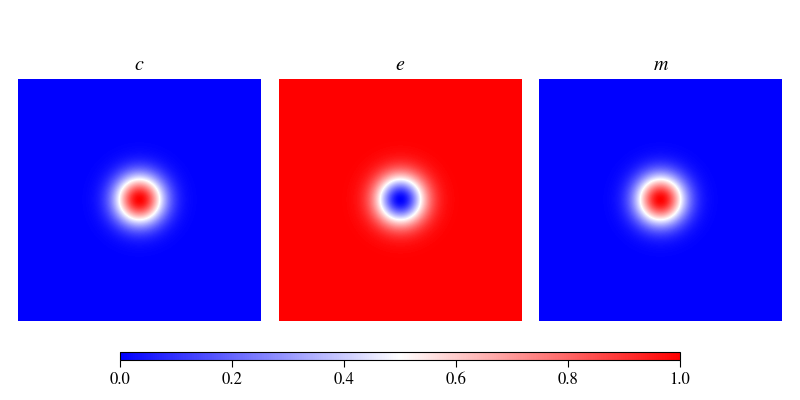
\includegraphics[width=\textwidth]{resources/images/2D_initial_conditions_homogenous_ECM.png}
    \caption{Visualization of the initial value distribution for an experiment in two space dimensions with a homogenous extracellular matrix}
    \label{fig:2D_homogenous_ECM_initial}
\end{figure}
Figure~\ref{fig:2D_homogenous_ECM_initial} shows a 2D plot of the initial conditions using the homogenous extracellular matrix structure. The images describing the tumor cell density and the matrix-degrading enzyme concentration have high values in the center. The image describing the extracellular matrix has high values everywhere except the center since the matrix-degrading enzymes have already degraded the ECM.


The other case we are investigating is using a heterogenous structured extracellular matrix. In section~\ref{sec:2D_heterogenous}, we investigate how a more realistic structure of the ECM will affect the results of a 2D simulation. Since we are looking at a heterogenous extracellular matrix only for in experiments with two spacial dimensions we are stating the initial conditions one the variable $e$ also for two spatial dimensions. For this scenario, we also assume a nodule of tumor cells in the center of the simulation that has produced a concentration of matrix-degrading enzymes. Contrary to the homogenous ECM strucutre, we assume that the tumor cells are located at a basement membrane that they already have invaded and are now pushing into the extracellular matrix behind it, located on the left side looking from the center. These assumptions are described in figure~\ref{fig:tumour_invasion_stage}. While the initial conditions on tumor cell density and matrix-degrading enzyme concentration are the same for both cases of ECM strucutre, we have to change the initial values of the variable $e$ to the following:
\begin{align*}
    e(x,y,0) = (1 - 0.5 \exp(-\frac{(x-0.5)^2+(y-0.5)^2+(z-0.5)^2}{0.01}))\frac{1}{1+\exp(-\frac{2}{0.1 (x-0.5)})}
\end{align*}

\begin{figure}[h]
    \centering
    \label{fig:Initial_Value_Distribution}
    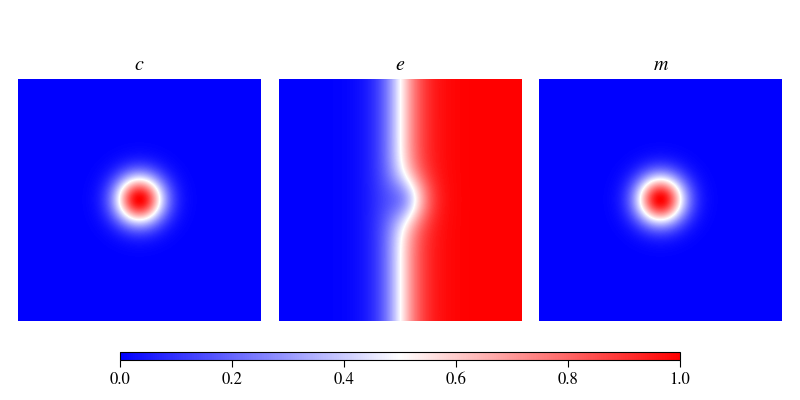
\includegraphics[width=\textwidth]{resources/images/2D_initial_conditions_heterogenous_ECM.png}
    \caption{Visualization of the initial value distribution for an experiment in two space dimensions with a heterogenous extracellular matrix}
    \label{fig:2D_heterogenous_ECM_initial}
\end{figure}
Figure~\ref{fig:2D_heterogenous_ECM_initial} describes these modifications on $e$ and shows the inital conditions for our system using a heterogenous ECM structure.
  


\subsection{Dimension Variation}

Before starting with the Parameter Analysis, we need to discuss how changing the dimension varies the results and what adjustments we need to take, to make our model mimick the one given by Anderson et al. Therefore we start with using the parameters given by Anderson et al.'s first experiment~\cite{anderson_mathematical_2000}. Figure~\ref{fig:anderson_experiment} shows a screenshot of this experiment, unfortunately in low resolution, since the original paper had not included any digital data containing the diagrams of their results.
\begin{figure}[ht!]
 \centering
 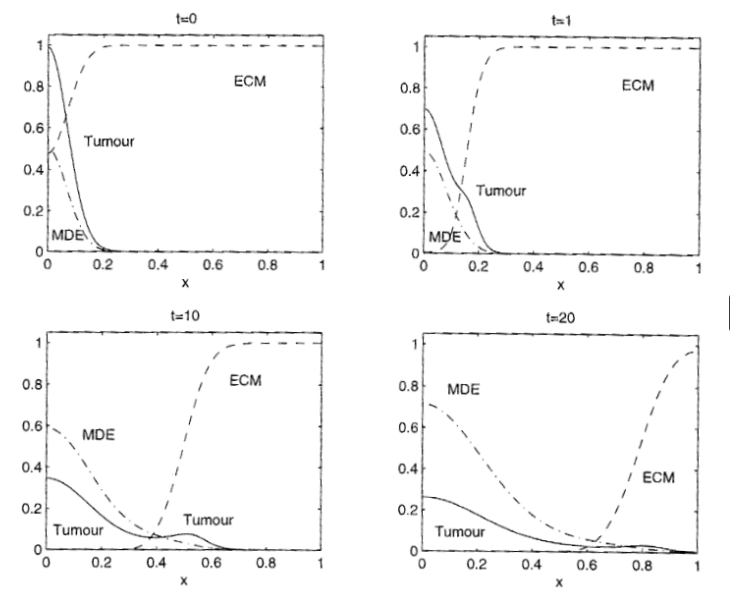
\includegraphics[width=\textwidth]{resources/images/anderson_experiment.png}
 \caption{Andersons first one dimensional experiment using the parameter values $d_c = 1\cdot 10^{-3}, d_m = 1\cdot 10^{-3}, \gamma = 0.005, \eta = 10, \alpha = 0.1, \beta = 0, \mu_1 = 0, \mu_2 = 0$}
 \label{fig:anderson_experiment}
\end{figure}
In the figure, you can see that after $t=1$ in their timescale, the tumor cells develop a division at the part invading the tissue. This division propagates to a pointy peak at a later point in time. The concentration of the matrix-degrading enzymes increases continuously and the concentration of the extracellular matrix decreases continuously. Their $x$-axis is stretched or rescaled to show an interval from $0$ to $1$. In our case, the interval on the plots has only $x$-values from $0$ to $0.5$.

\begin{figure}[ht!]
 \centering
 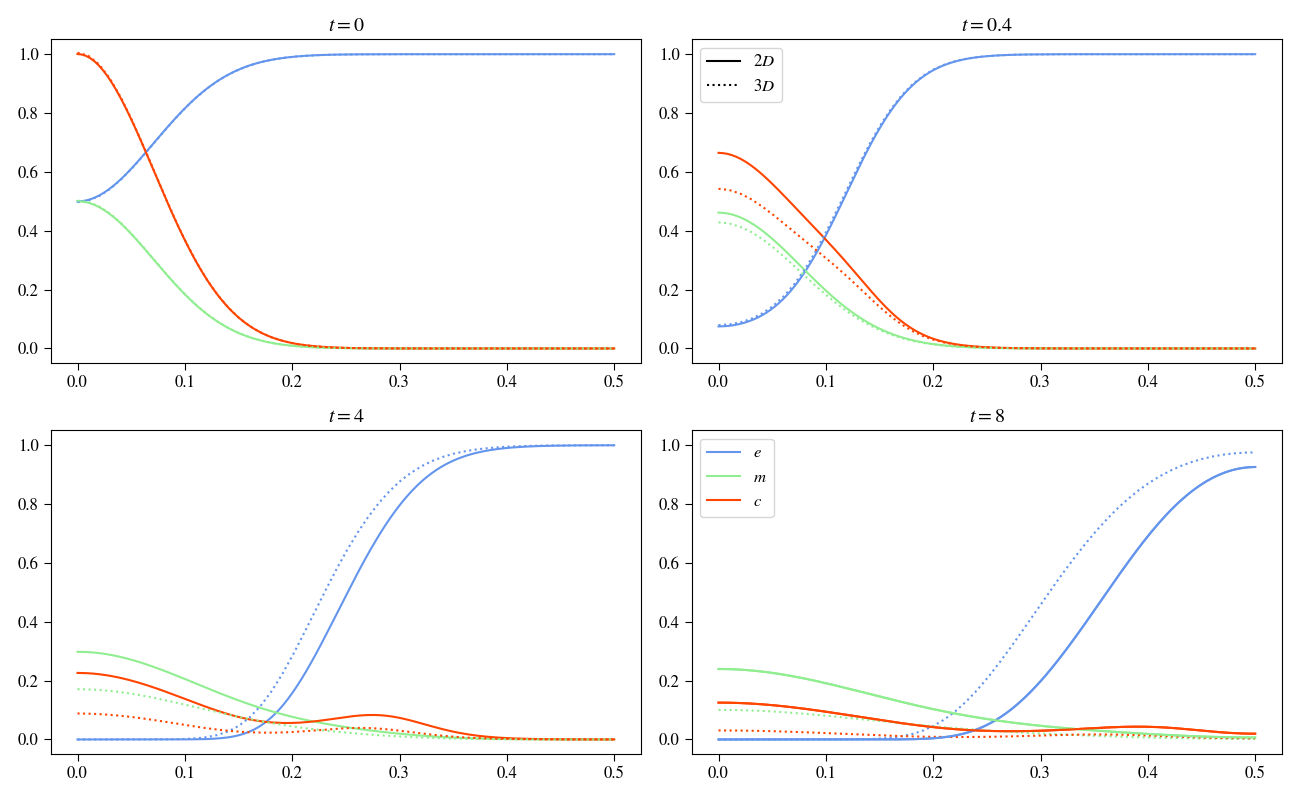
\includegraphics[width=\textwidth]{resources/images/1D_replication_3D.png}
 \caption{Results using Anderson et al.'s parameters produced by applying the Plot Over Line tool in two and three dimensions}
 \label{fig:unadjsuted_replication}
\end{figure}

Replicating this experiment in two and three dimensions, we start with the same parameters as Anderson et al. had used, $d_c = 1\cdot 10^{-3}, d_m = 1\cdot 10^{-3}, \gamma = 0.005, \eta = 10, \alpha = 0.1, \beta = 0$. Figure~\ref{fig:unadjsuted_replication} and adjust them to make our simulation match Anderson et al.'s as good as possible. 

Starting from the initial values, we see that after $t=0.4$, a very small division of the tumor cells is starting to form for both dimensions. This division increases strongly for the experiment done in two dimensions and minimal for the experiment done in three dimensions at $t=4$. At $t=8$, both curves visibly flatten. We see that the division of tumor cells detaching from the primary tumor are not as pregnant as in the one-dimensional experiment of Anderson et al. The interplay of the diffusive and haptotatic factors determines how considerable this division will be that detaches from the primary lump of the tumor cells and invades the tissue faster. It will also decide how pointy this secondary lump of tumor cells will be. Biologically, this relation between diffusion and haptotaxis translates to the invasion pace of the tumor cells, the rate at which how much of them will remain at the primary tumor and how much will invade further into the tissue degrading the extracellular matrix.

Looking at the concentration of matrix-degrading enzymes, we see it is visibly lower here than in Anderson et al.'s experiment. We see little increase over time. We can change this by changing the production factor of $\alpha$ or by adjusting the motility of the tumor cells producing them exponentially. The factor $\alpha$ determines how fast the tumor cells produce the matrix-degrading enzymes, degrading the extracellular matrix and allowing the tumor cells to invade the tissue further.

Only the extracellular matrix concentration seems to mimic the behavior of Anderson et al.'s experiment. It decreases continuously and as the last image shows, there is still a considerable amount left.

To replicate Anderson et al.'s results, we will start adjusting the parameters mentioned exemplary in two spacial dimensions: the tumor cells' diffusion and haptotxis coefficients and the production rate of the matrix-degrading enzymes. We are focusing on the values the variables will take at the origin $x=0$. Since Anderson et al. used in the original paper the model without tumor cell proliferation and extracellular matrix renewal, we are using the same model during the dimensional variation.

\begin{figure}[!htb]
 \centering
 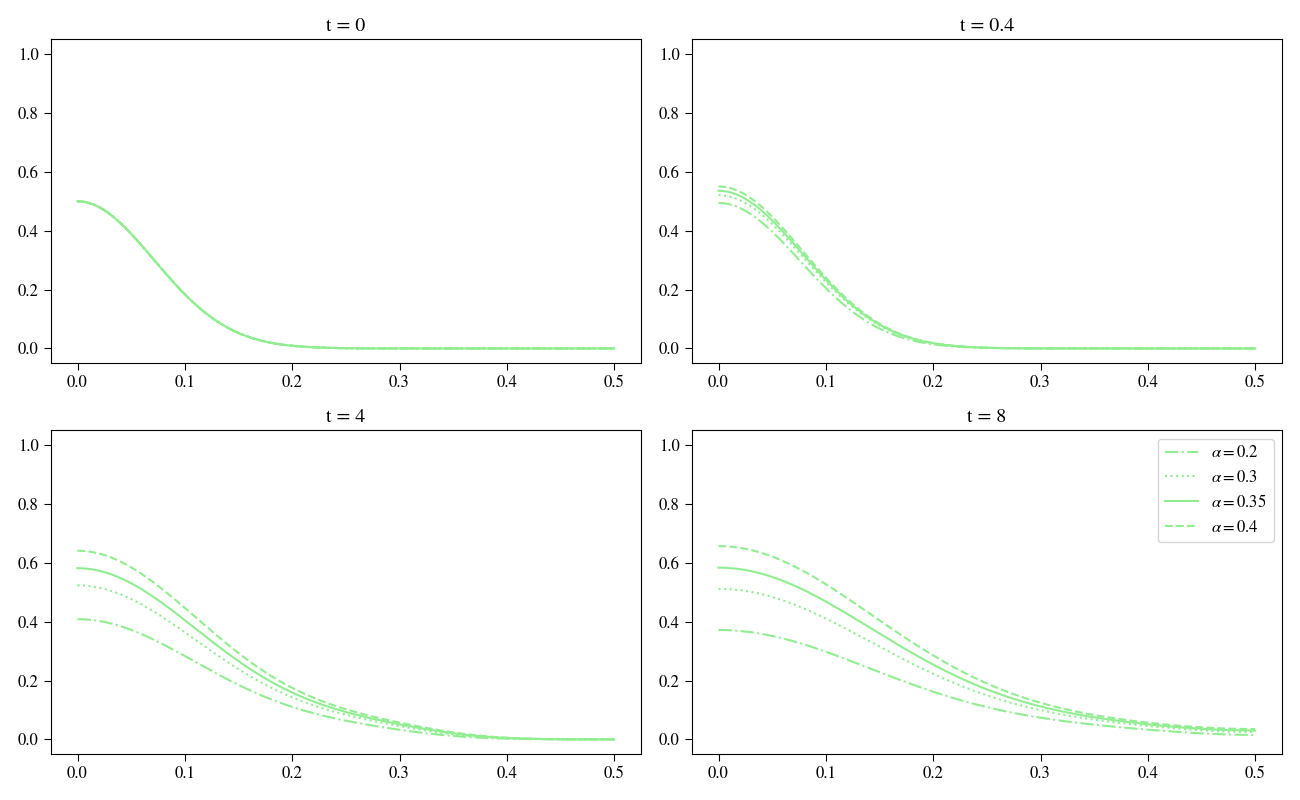
\includegraphics[width=\textwidth]{resources/images/alpha_comparison.png}
 \caption{Comparison of $\alpha$ values to replicate Anderson et al.'s experiment}
 \label{fig:replication_alpha_comparison}
\end{figure}

Starting with comparing different values for $\alpha$, we see in figure~\ref{fig:replication_alpha_comparison} a comparison of how this affects the curve for the matrix-degrading enzyme concentration. A maximum difference between the compared values of $0.2$ already causes drastic changes. In Anderson et al.'s experiment, we observed a value of approximately $m(0,1)=0.5$ after, in their timescale, $t=1$ at the origin. This value is mimicked best for a value of $\alpha=0.2$ in our experiments. However, in the later points in time, we see that this value for $\alpha$ is insufficiently low in terms of increase, though choosing $\alpha$ higher than $\alpha=0.4$ results in an accelerated ECM degradation that is too fast. Taking a value between those two allowed our simulations to exhibit the observed behavior. We choose a value of $\alpha=0.35645$ to use in the later experiments as a basecase.

\begin{figure}[!htb]
 \centering
 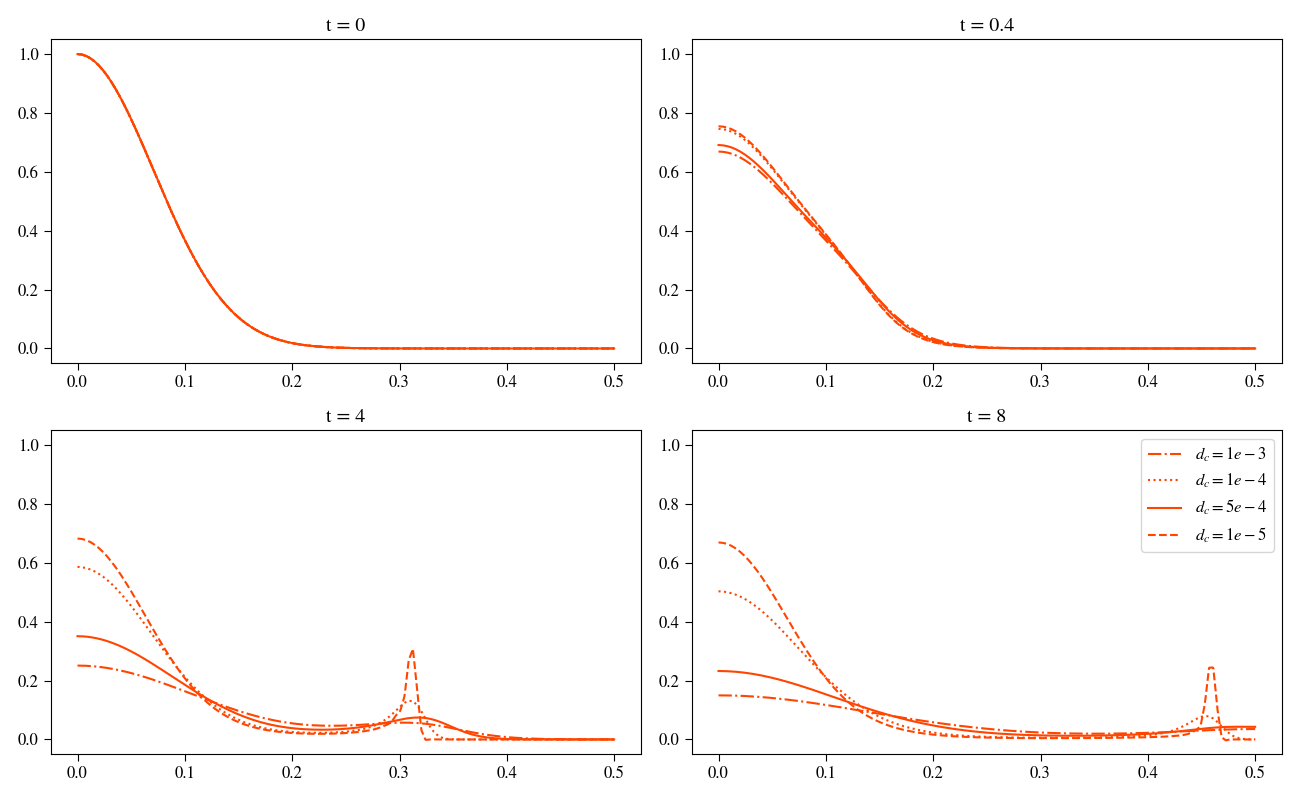
\includegraphics[width=\textwidth]{resources/images/dc_comparison.png}
 \caption{Comparison of $d_c$ values to replicate Anderson et al.'s experiment}
 \label{fig:replication_dc_comparison}
\end{figure}

Looking at the diffusion coefficient for the tumor cells, in figure~\ref{fig:replication_dc_comparison}, you can see different $d_c$ values regarding the tumor cell concentration. It is clear that with decreasing $d_c$, the sharpness of the secondary lump of cells that begins to invade the tissue drastically increases due to increased effects of haptotaxis, which is now the main factor in controlling tumor motility. However, we also observe that with decreasing $d_c$, the remaining lump of tumor cells at the origin increases due to little diffusion here. Over time, we found that $dc=5 \cdot 10^{-4}$ describes Anderson et al.'s experimental results best for our simulations, with a roughly matching density of tumor cells that remains at the origin at all times and, for our case, balanced effects of haptotaxis and diffusion.

\begin{figure}[!htb]
 \centering
 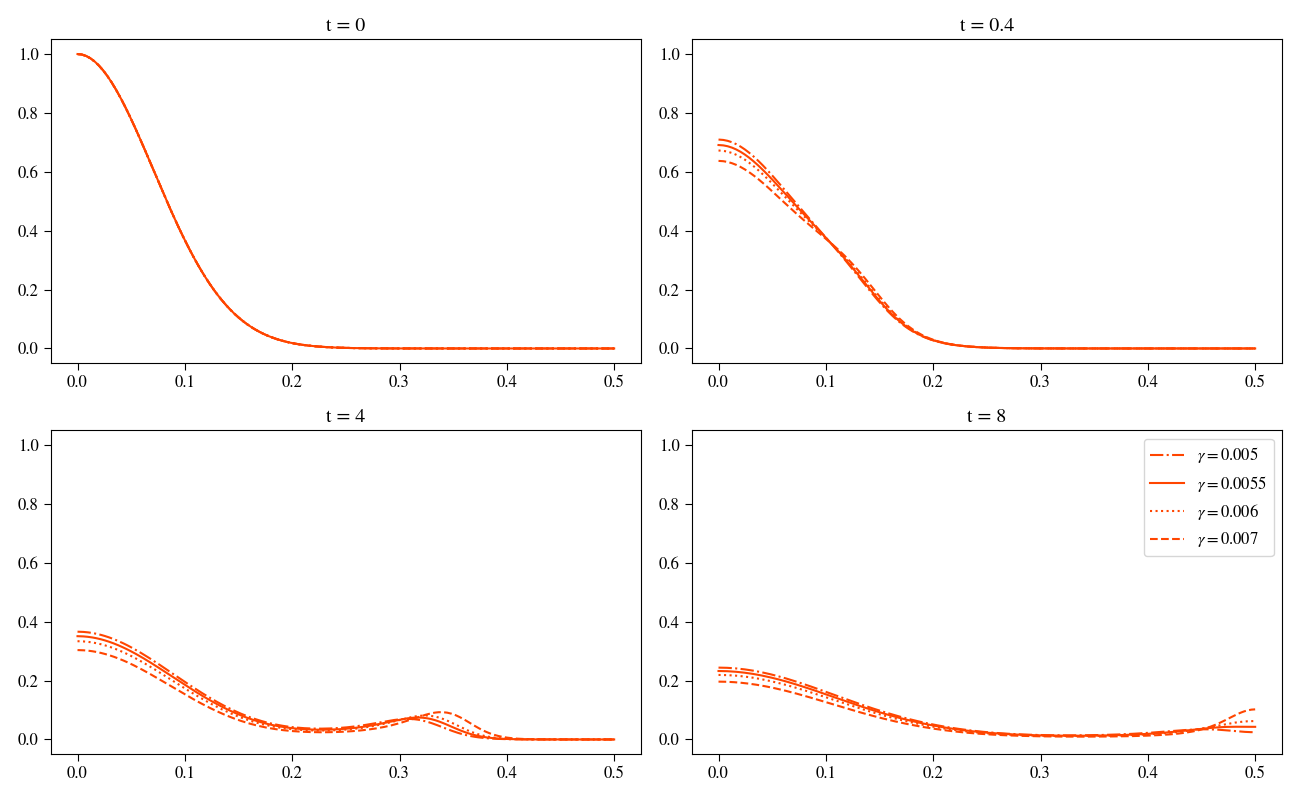
\includegraphics[width=\textwidth]{resources/images/gamma_comparison.png}
 \caption{Comparison of $\gamma$ values to replicate Anderson et al.'s experiment}
 \label{fig:replication_gamma_comparison}
\end{figure}

At last, we want to adjust the haptotatic pull slightly; for this, we are looking at a comparison of different $\gamma$ values in figure~\ref{fig:replication_gamma_comparison} depicting the tumor cell density. Comparing our results with Anderson et al.'s, we want a bigger secondary lump that invades the tumor cells faster than the one remaining at the origin. We need to increase $\gamma$ to increase the haptotatic pull that controls tumor cell motility. The figure shows that increasing $\gamma$ yields these effects, but increasing it too much results in a too-fast invasion pace of the surrounding tissue. Increasing $\gamma$ slightly to $\gamma=0.0055$ is sufficient to produce the desired effects.

\begin{figure}[h!]
    \centering
    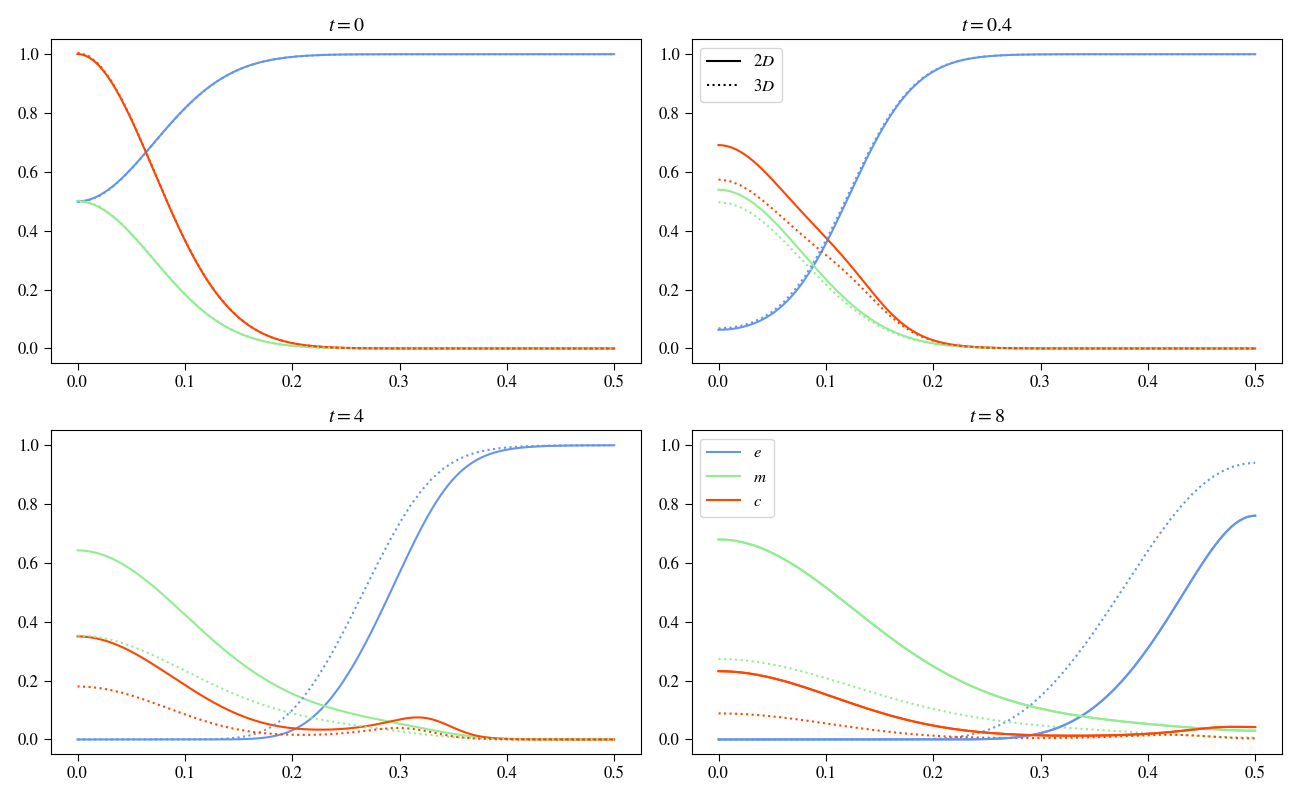
\includegraphics[width=\textwidth]{resources/images/2D_without_proliferation_replication_3D.png}
    \caption{3D Replication of using the 2D basecases values}
    \label{fig:2D_proliferation_replication_3D}
\end{figure}

These adjustments leave us with the final configuration for replicating the system in two dimensions. We see the important effects met when comparing the two dimensional experiment with the original experiment. We see that the production of the matrix-degrading enzymes fits the original experiment and the motility of the tumor cells also matches, with balanced effects of haptotaxis and diffusion. However comparing the three-dimensional experiment to original, there are still major differences. The second timestep $t=0.4$ shows a tumor cell density that is considerably lower in the 3D experiment than in the 2D experiment, which is can also be observed at the later points in time. Due to the exponential production of matrix-degrading enzymes by the tumor cells, the change in tumor cell density also effects the MDE concentration massively, resulting also in a lower concentration. The also reduced MDE concentration causes a slower degradation process of the extracellular matrix.

\begin{figure}[h!]
    \centering
    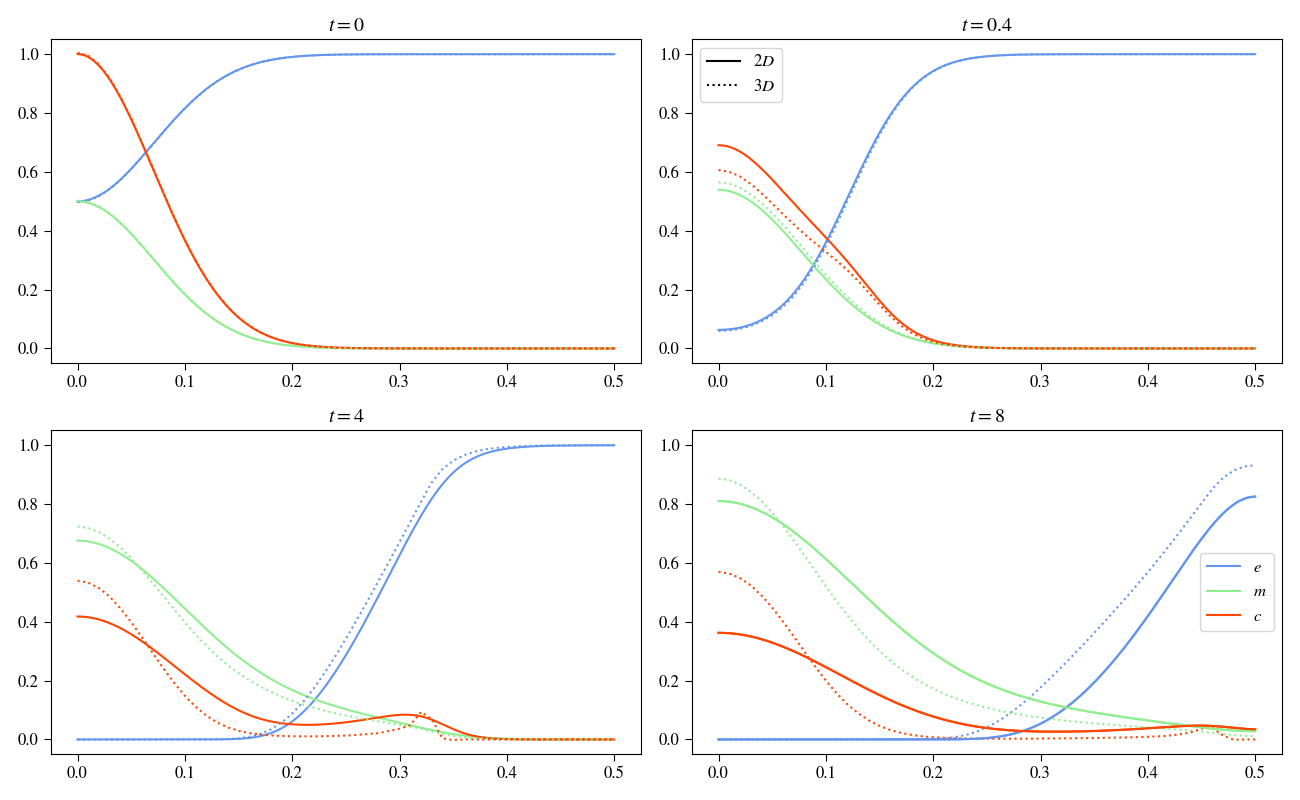
\includegraphics[width=\textwidth]{resources/images/basecase_replication.png}
    \caption{Comparing 2D basecase with proliferation and 3D basecase for proliferation}
    \label{fig:3D_basecase_comparison}
\end{figure}

In figure~\ref{fig:3D_basecase_comparison}, we used the same scematic we did above, changing $d_c,\gamma$ and $\alpha$ to make the 3D results simulations match the results produced in 2D or 1D. Challenging in this process was, as mentioned previously, that the reduced tumor cell density causes drastic changes in both MDE production and ECM degradation. Settling on the values: $d_c=3 \cdot 10{-4}, \gamma=0.0058, \alpha=0.6$, yields sufficiently matching results.

Now the question arises why we have to change those values to replicate results. We can argue here with the parameter analysis, but also with an algebraic hypothesis. 

Since $\beta$ is assumed for most experiments to be zero, also in repilication one-dimensional results in two dimensions, we also set it to zero in this case. 

Looking at the parameter analysis for $d_m$ we saw that this parameter has litlle influence compared to other on the simulation, excepting the overall MDE concentration in certain regions, which is neglectable when in those regions the ECM is already fully degraded. Also regarding the spacial occupation and distribution of the matrix-degrading enzymes we saw that a more important factor is the motility of the tumor cells producing them in their wake. 

Inspecting the term concerning $\eta$ we see that it depends on local values for the ECM and MDE concentrations; $-\eta m(x,y,z,t)e(x,y,z,t)$. In the expereiments regarding replicating we see that we can influence the MDE concentration well with adjusting the motility of the tumor cells and their production of the MDEs. In figure~\ref{fig:3D_basecase_comparison} you see that the concentration of the matrix-degrading enzymes roughly matches over time for both dimensions. In the plots $m(x,y,z,t)e(x,y,z,t)$ therefore also roughly match, resulting in similar ECM degradation rate. Becasue of this, we also do not change $\eta$.

As mentioned above the tumor cell motility plays a cruical role during temporal developement of the whole system. It is therefore a key component to match these curves. The motility is goverened by diffusion and haptotaxis: 
\begin{align*}
    d_c\Delta c - \gamma \nabla\cdot (c\nabla e)=d_c\Delta c - \gamma (\nabla c \cdot \nabla e + \Delta e)
\end{align*}.

\begin{table}[htbp]
    \centering
    \begin{tabular}{|c|c|c|c|}
        \hline
        & $1D$ & $2D$ & $3D$ \\ 
        \hline
        Diffusion & $\frac{\partial^{2}c}{\partial x^{2}}$ & $\frac{\partial^{2}c}{\partial x^{2}}+\frac{\partial^{2}c}{\partial y^{2}}$ & $\frac{\partial^{2}c}{\partial x^{2}}+\frac{\partial^{2}c}{\partial y^{2}}+\frac{\partial^{2}c}{\partial z^{2}}$\\
        \hline
        Haptotaxis & $\frac{\partial c}{\partial x}\frac{\partial e}{\partial x} + \frac{\partial^{2}e}{\partial x^{2}}$ & $\frac{\partial c}{\partial x}\frac{\partial e}{\partial x} + \frac{\partial c}{\partial y} \frac{\partial e}{\partial y} + \frac{\partial^{2}e}{\partial x^{2}} + \frac{\partial^{2}e}{\partial y^{2}} $ & $\frac{\partial c}{\partial x}\frac{\partial e}{\partial x} + \frac{\partial c}{\partial y}\frac{\partial e}{\partial y} + \frac{\partial c}{\partial z}\frac{\partial e}{\partial z} + \frac{\partial^{2}e}{\partial x^{2}} + \frac{\partial^{2}e}{\partial y^{2}} + \frac{\partial^{2}e}{\partial z^{2}}$ \\
        \hline
    \end{tabular}
    \caption{Overview of Diffusion and Haptotaxis terms across varying dimensions}
    \label{tab:diff_hapto}
\end{table}
Table~\ref{tab:diff_hapto} gives an overview of the diffusion and haptotaxis terms for the treated dimensions in this work. For the diffusion we see that with increasing the dimension we get one additional term, assuming for simplicity $\frac{\partial^{2}c}{\partial x^{2}}=\frac{\partial^{2}c}{\partial y^{2}}=\frac{\partial^{2}c}{\partial z^{2}}=\kappa(t)$. Also assuming a constant factor $M$ for diffusion, this yields in one spacial dimension $M=d_{c,1}\kappa(t)$, equivalent to $d_{c,1}=\frac{M}{\kappa(t)}=1\cdot 10^{-3}$; in two spacial dimensions $d_{c,2}=\frac{M}{2\kappa(t)}=\frac{1}{2}d_{c,1}=\frac{1}{2} 10^{-3}=5 \cdot 10^{-4}$ and in three dimensions $d_{c,3}=\frac{M}{3\kappa(t)}=\frac{1}{3}d_{c,1}=\frac{1}{3} 10^{-3}=3.33 \cdot 10^{-4}$. 

If we applied the same hypothesis for $\gamma$; assuming a constant factor $H$ for it and assuming $\frac{\partial c}{\partial x}\frac{\partial e}{\partial x}=\frac{\partial c}{\partial y}\frac{\partial e}{\partial y}=\frac{\partial c}{\partial z}\frac{\partial e}{\partial z}=\iota$, $\frac{\partial^{2}e}{\partial x^{2}}=\frac{\partial^{2}e}{\partial y^{2}}=\frac{\partial^{2}e}{\partial z^{2}}=\theta$, we would get in one dimension: $\gamma_1 = \frac{H}{\iota + \kappa(t)} = 0.005$, in two: $\gamma_2 = \frac{H}{2\iota + 2\kappa(t)} = \frac{1}{2} \gamma_1 = 0.0025$ and in three dimensions: $\gamma_3 = \frac{H}{3\iota + 3\kappa(t)} = \frac{1}{3} \gamma_1 = 0.00166$. We see from experimental results that using $\gamma=0.002$ and $d_c=5\cdot 10^{-4}$ yields a curve for the tumor cells that has no secondary lump of cells detaching from  the primary tumor. Adjusting $\gamma$ we cannot employ the same hypothesis, since the equation describing haptotaxis also incorporates a term regarding the gradients of both curves; $\nabla c \cdot \nabla e$ not only the laplacian of the extracellular matrix concentratin $\Delta e$. Depending on the point in space and time we look at $\nabla c(x,y,z,t) \cdot \nabla e(x,y,z,t)$, this term can damping increasing or no effect at all. We therefore resort to determining this value experimentally with a value of $\gamma=0.0057$.

Further improvements to make the experiments match better could be made on varying $\mu_1$ and $\mu_2$ to either match the tumor cell density more acurately or the degradation rate of the extracellular matrix.

The conclusions we can draw from adjusting the parameters with varying the dimensions are that the most important factor is the tumor cell density. The motility is cruical for the as well the shape of the MDE curve as well as the concentration of it, due to the tumor cells producing them exponentially, but this we can also adjust with the production coefficient $\alpha$. Diffusion coefficient can be calculated algebraicly, as seen above, but for Haptotaxis the coefficient must be determined experimentally. It is to say that due though it is possible to make the simulations across dimensions match at one point in time, it is due to the many different parameters and terms impossible to make them perfeclty fit over time.


\begin{longtable}{|c c c c c c c c|}
    \hline
    Figure & Linestyle & $d_c$ & $\gamma$ & $\eta$ & $d_m$ & $\alpha$ & $\beta$ \\ [0.5ex] 
    \hline\hline
    \endfirsthead
    \hline
    Figure & Linestyle & $d_c$ & $\gamma$ & $\eta$ & $d_m$ & $\alpha$ & $\beta$ \\ [0.5ex] 
    \hline\hline
    \endhead
    \hline \multicolumn{8}{|r|}{{continued on next page}} \\ \hline
    \endfoot
    \endlastfoot
    \ref{fig:unadjsuted_replication} & \sampleline{} & $1\cdot 10^{-3}$ & $0.005$ & $10$& $1\cdot 10^{-3}$ & $0.1$ & $0$\\  \hline
    \ref{fig:replication_alpha_comparison} & \sampleline{dash pattern=on .7em off .2em on .05em off .2em} & $1\cdot 10^{-3}$ & 0.005 & 10 & $1\cdot 10^{-3}$ & 0.2 & 0\\  \hline
    \ref{fig:replication_alpha_comparison} & \sampleline{dotted} & $1\cdot 10^{-3}$ & 0.005 & 10 & $1\cdot 10^{-3}$ & 0.3 & 0\\  \hline
    \ref{fig:replication_alpha_comparison} & \sampleline{} & $1\cdot 10^{-3}$ & 0.005 & 10 & $1\cdot 10^{-3}$ & 0.35 & 0\\  \hline
    \ref{fig:replication_alpha_comparison} & \sampleline{dashed} & $1\cdot 10^{-3}$ & 0.005 & 10 & $1\cdot 10^{-3}$ & 0.4 & 0\\  \hline
    \ref{fig:replication_dc_comparison} & \sampleline{dash pattern=on .7em off .2em on .05em off .2em} & $1\cdot 10^{-3}$ & 0.005 & 10 & $1\cdot 10^{-3}$ & 0.3546 & 0\\  \hline
    \ref{fig:replication_dc_comparison} & \sampleline{dotted} & $1\cdot 10^{-4}$ & 0.005 & 10 & $1\cdot 10^{-3}$ & 0.3546 & 0\\  \hline
    \ref{fig:replication_dc_comparison} & \sampleline{} & $5\cdot 10^{-4}$ & 0.005 & 10 & $1\cdot 10^{-3}$ & 0.3546 & 0\\  \hline
    \ref{fig:replication_dc_comparison} & \sampleline{dashed} & $1\cdot 10^{-5}$ & 0.005 & 10 & $1\cdot 10^{-3}$ & 0.3546 & 0\\  \hline
    \ref{fig:replication_gamma_comparison} & \sampleline{dash pattern=on .7em off .2em on .05em off .2em} & $5\cdot 10^{-5}$ & 0.005 & 10 & $1\cdot 10^{-3}$ & 0.3546 & 0\\  \hline
    \ref{fig:replication_gamma_comparison} & \sampleline{dotted} & $5\cdot 10^{-4}$ & 0.0055 & 10 & $1\cdot 10^{-3}$ & 0.3546 & 0\\  \hline
    \ref{fig:replication_gamma_comparison} & \sampleline{} & $5\cdot 10^{-4}$ & 0.006 & 10 & $1\cdot 10^{-3}$ & 0.3546 & 0\\  \hline
    \ref{fig:replication_gamma_comparison} & \sampleline{dashed} & $5\cdot 10^{-4}$ & 0.007 & 10 & $1\cdot 10^{-3}$ & 0.3546 & 0\\  \hline
    \ref{fig:2D_proliferation_replication_3D} & \sampleline{} & $5\cdot 10^{-4}$ & 0.0055 & 10 & $1\cdot 10^{-3}$ & 0.3546 & 0\\  \hline
    \ref{fig:2D_proliferation_replication_3D} & \sampleline{dotted} & $5\cdot 10^{-4}$ & 0.0055 & 10 & $1\cdot 10^{-3}$ & 0.3546 & 0\\  \hline
    \ref{fig:3D_basecase_comparison} & \sampleline{} & $5\cdot 10^{-4}$ & 0.0055 & 10 & $1\cdot 10^{-3}$ & 0.3546 & 0\\  \hline
    \ref{fig:3D_basecase_comparison} & \sampleline{} & $3.3\cdot 10^{-4}$ & 0.0058 & 10 & $1\cdot 10^{-3}$ & 0.6 & 0\\  \hline
    \caption{Overview of all experiments conducted for the model without proliferation and renewal producing 2D output}
    \label{table:replication_experiments}
\end{longtable}

In table~\ref{table:replication_experiments} all experiments with their corresponding parameter configurations and linestyles in the respective figures are listed.



\subsection{Parameter Analysis without Proliferation and Renewal - Homogenous ECM}
\label{sec:2D_without_proliferation}

This section describes the Parameter Analysis done in two spacial dimensions on a homogenous extracellular matrix structure. In this section we are using the basecase for established in the previous section with the parameters as used in~\ref{fig:2D_proliferation_replication_3D}. 

\begin{longtable}{|c c c c c c c c|}
    \hline
    Figure & Linestyle & $d_c$ & $\gamma$ & $\eta$ & $d_m$ & $\alpha$ & $\beta$ \\ [0.5ex] 
    \hline\hline
    \endfirsthead
    \hline
    Figure & Linestyle & $d_c$ & $\gamma$ & $\eta$ & $d_m$ & $\alpha$ & $\beta$ \\ [0.5ex] 
    \hline\hline
    \endhead
    \hline \multicolumn{8}{|r|}{{continued on next page}} \\ \hline
    \endfoot
    \endlastfoot
    \ref{fig:dc_variation} & \sampleline{} & $1\cdot 10^{-4}$ & 0.0055 & 10 & $1\cdot 10^{-3}$ & 0.3546 & 0\\ \hline
    \ref{fig:dc_variation} & \sampleline{dotted} & $1\cdot 10^{-3}$ & 0.0055 & 10 & $1\cdot 10^{-3}$ & 0.3546 & 0\\ \hline
    \ref{fig:gamma_variation} & \sampleline{dotted} & $5\cdot 10^{-4}$ & 0.002 & 10 & $1\cdot 10^{-3}$ & 0.3546 & 0\\ \hline
    \ref{fig:gamma_variation} & \sampleline{} & $5\cdot 10^{-4}$ & 0.008 & 10 & $1\cdot 10^{-3}$ & 0.3546 & 0\\ \hline
    \ref{fig:gamma_variation} & \sampleline{dashed} & $5\cdot 10^{-4}$ & 0.01 & 10 & $1\cdot 10^{-3}$ & 0.3546 & 0\\ \hline
    \ref{fig:gamma_2D_plot} & \sampleline{} & $5\cdot 10^{-4}$ & 0.1 & 10 & $1\cdot 10^{-3}$ & 0.3546 & 0\\ \hline
    \ref{fig:eta_variation} & \sampleline{dotted} & $5\cdot 10^{-4}$ & 0.0055 & 2 & $1\cdot 10^{-3}$ & 0.3546 & 0\\ \hline
    \ref{fig:eta_variation} & \sampleline{} & $5\cdot 10^{-4}$ & 0.0055 & 12 & $1\cdot 10^{-3}$ & 0.3546 & 0 \\ \hline
    \ref{fig:eta_variation} & \sampleline{dotted} & $5\cdot 10^{-4}$ & 0.0055 & 20 & $1\cdot 10^{-3}$ & 0.3546 & 0 \\ \hline
    \ref{fig:dm_variation} & \sampleline{dotted} & $1\cdot 10^{-3}$ & 0.0055 & 10 & 0.00001 & 0.3546 & 0 \\ \hline
    \ref{fig:dm_variation} & \sampleline{} & $1\cdot 10^{-4}$ & 0.0055 & 10 & 0.001 & 0.3546 & 0 \\ \hline
    \ref{fig:dm_variation} & \sampleline{dashed} & $1\cdot 10^{-5}$ & 0.0055 & 10 & 0.1 & 0.3546 & 0 \\ \hline
    \ref{fig:alpha_variation} & \sampleline{dotted} & $5\cdot 10^{-4}$ & 0.0055 & 10 & $1\cdot 10^{-3}$ & 0 & 0 \\ \hline
    \ref{fig:alpha_variation} & \sampleline{} & $5\cdot 10^{-4}$ & 0.0055 & 10 & $1\cdot 10^{-3}$ & 0.6 & 0 \\ \hline
    \ref{fig:alpha_variation} & \sampleline{dotted} & $5\cdot 10^{-4}$ & 0.0055 & 10 & $1\cdot 10^{-3}$ & 1.0 & 0 \\ \hline
    \ref{fig:beta_variation} & \sampleline{dotted} & $5\cdot 10^{-4}$ & 0.0055 & 10 & $1\cdot 10^{-3}$ & 0.3546 & 0.1 \\ \hline
    \ref{fig:beta_variation} & \sampleline{} & $5\cdot 10^{-4}$ & 0.0055 & 10 & $1\cdot 10^{-3}$ & 0.3546 & 0.01 \\ \hline
    \ref{fig:beta_variation} & \sampleline{dotted} & $5\cdot 10^{-4}$ & 0.0055 & 10 & $1\cdot 10^{-3}$ & 0.3546 & 0.005 \\ \hline
    \ref{fig:dc_gamma_variation} - left& \sampleline{dotted} & $5\cdot 10^{-5}$ & 0.001 & 10 & $1\cdot 10^{-3}$ & 0.3546 & 0 \\ \hline
    \ref{fig:dc_gamma_variation} - left & \sampleline{} & $5\cdot 10^{-5}$ & 0.01 & 10 & $1\cdot 10^{-3}$ & 0.3546 & 0 \\ \hline
    \ref{fig:dc_gamma_variation} -right & \sampleline{dotted} & $1\cdot 10^{-3}$ & 0.001 & 10 & $1\cdot 10^{-3}$ & 0.3546 & 0 \\ \hline
    \ref{fig:dc_gamma_variation} -right & \sampleline{} & $1\cdot 10^{-3}$ & 0.01 & 10 & $1\cdot 10^{-3}$ & 0.3546 & 0 \\ \hline
    \ref{fig:dm_eta_variation} - left & \sampleline{dotted} & $5\cdot 10^{-4}$ & 0.0055 & 2 & $1\cdot 10^{-5}$ & 0.3546 & 0 \\ \hline
    \ref{fig:dm_eta_variation} - left & \sampleline{} & $5\cdot 10^{-4}$ & 0.0055 & 20 & $1\cdot 10^{-5}$ & 0.3546 & 0 \\ \hline
    \ref{fig:dm_eta_variation} -right & \sampleline{dotted} & $5\cdot 10^{-4}$ & 0.0055 & 2 & $1\cdot 10^{-3}$ & 0.3546 & 0 \\ \hline
    \ref{fig:dm_eta_variation} -right & \sampleline{} & $5\cdot 10^{-4}$ & 0.0055 & 20 & $1\cdot 10^{-3}$ & 0.3546 & 0 \\ \hline
    \ref{fig:alpha_beta_variation} - left & \sampleline{dotted} & $5\cdot 10^{-4}$ & 0.0055 & 10 & $1\cdot 10^{-3}$ & 0.1 & 0.005 \\ \hline
    \ref{fig:alpha_beta_variation} - left & \sampleline{} & $5\cdot 10^{-4}$ & 0.0055 & 10 & $1\cdot 10^{-3}$ & 0.1 & 0.1 \\ \hline
    \ref{fig:alpha_beta_variation} -right & \sampleline{dotted} & $5\cdot 10^{-4}$ & 0.0055 & 10 & $1\cdot 10^{-3}$ & 1.0 & 0.005 \\ \hline
    \ref{fig:alpha_beta_variation} -right & \sampleline{} & $5\cdot 10^{-4}$ & 0.0055 & 10 & $1\cdot 10^{-3}$ & 1.0 & 0.1 \\ \hline
    \ref{fig:dm_alpha_beta_variation_1} - left & \sampleline{dotted} & $5\cdot 10^{-4}$ & 0.0055 & 10 & $1\cdot 10^{-5}$ & 0.1 & 0.005 \\ \hline
    \ref{fig:dm_alpha_beta_variation_1} - left & \sampleline{} & $5\cdot 10^{-4}$ & 0.0055 & 10 & $1\cdot 10^{-5}$ & 0.1 & 0.1 \\ \hline
    \ref{fig:dm_alpha_beta_variation_1} -right & \sampleline{dotted} & $5\cdot 10^{-4}$ & 0.0055 & 10 & $1\cdot 10^{-5}$ & 1.0 & 0.005 \\ \hline
    \ref{fig:dm_alpha_beta_variation_1} -right & \sampleline{} & $5\cdot 10^{-4}$ & 0.0055 & 10 & $1\cdot 10^{-5}$ & 1.0 & 0.1 \\ \hline
    \ref{fig:dm_alpha_beta_variation_2} - left & \sampleline{dotted} & $5\cdot 10^{-4}$ & 0.0055 & 10 & $1\cdot 10^{-3}$ & 0.1 & 0.005 \\ \hline
    \ref{fig:dm_alpha_beta_variation_2} - left & \sampleline{} & $5\cdot 10^{-4}$ & 0.0055 & 10 & $1\cdot 10^{-3}$ & 0.1 & 0.1 \\ \hline
    \ref{fig:dm_alpha_beta_variation_2} -right & \sampleline{dotted} & $5\cdot 10^{-4}$ & 0.0055 & 10 & $1\cdot 10^{-3}$ & 1.0 & 0.005 \\ \hline
    \ref{fig:dm_alpha_beta_variation_2} -right & \sampleline{} & $5\cdot 10^{-4}$ & 0.0055 & 10 & $1\cdot 10^{-3}$ & 1.0 & 0.1 \\ \hline
    \caption{Overview of all experiments conducted for the model without proliferation and renewal producing 2D output}
    \label{table:2D_experiments_without_proliferation}
\end{longtable}
Table~\ref{table:2D_experiments_without_proliferation} gives a detailed overview of all the experiments done in this section and the parameters used to produce the results. We are considering the model without the proliferation of the tumor cells or renewal of the extracellular matrix. Therefore, parameters $\mu_1$ and $\mu_2$ are set to zero. In most figures, more than one experiment will be described; the linestyle in table~\ref{table:2D_experiments_without_proliferation} determines which experiment exactly is described by the set of parameters.


\subsubsection{Parameter Analysis}
Before we start with the parameter analysis, we will discuss the mathematical intuition concerning the system of partial differential equations, equations~\ref{eq:6} to~\ref{eq:10}. 

The equation governing the tumor cell density incorporates only two coefficients in this version regarding its motility, diffusion and haptotaxis. As mentioned during replicating Anderson et al.'s experiment, the relation between those two factors determines if a secondary lump of tumor cells detaches from the main lump and invades the tissue faster than the remaining cells but also how large this lump will be. We saw this behaviour in figure~\ref{fig:replication_dc_comparison}, varying $d_c$ whilst keeping $\gamma$ constant. Diffusive motility depends on the laplacian of the tumor cells themselves, $\Delta c = \frac{\partial c}{\partial x} + \frac{\partial c}{\partial y} + \frac{\partial c}{\partial z}$, which is a fundamental tool in sciences of all sorts to describe the effects of spacial rate of change of a scalar field quantity, in our case tumor cell density, at a specific point in space. Typically, this operator has high values where the respective quantity changes rapidly. We have a similar haptotaxis term: $\nabla \cdot (c\nabla e) = \nabla c \cdot \nabla e + \Delta e$. This relation means that haptotatic effects are strong not only where the concentration of the extracellular matrix changes rapidly but also where both gradients for tumor cell density and extracellular matrix assimilate in direction. However, these effects can also annihilate each other.

The equation describing the concentration of the extracellular matrix models its exponential decay, taking the concentration of the matrix-degrading enzymes into account. In spatial and temporal positions where both ECM and MDE concentrations are high, we can expect a fast degradation of the extracellular matrix.

The equation modeling the matrix-degrading enzymes combines motility with production/decay terms. The motility of the MDEs is modeled by the same diffusion as the tumor cells, mimicking their behavior in this regard. The tumor cells are responsible for producing the MDEs; the production is modeled by natural decay and both production and decay are modeled using exponential approaches.

From the replicated results shown in figure~\ref{fig:basecase_without_proliferation}, we saw that the results can vary strongly if we vary the parameters one at a time. We will first look at how changing one parameter at a time affects the output of the simulation. After this, we will consider changing multiple parameters simultaneously in the cross-variation section. For varying the parameters, we assume the other parameters of the system are constant and use the baseline experiment as their values.

\subsubsection*{$d_c$ Variation}
This parameter describes the diffusive properties of the tumor cells. As Chaplain et al. assumed in~\cite{STEPHANOU200696}, we are also assuming an even distribution of this parameter with $d_c \sim U[1\cdot 10^{-5}, 1\cdot 10^{-3}]$. However, our experiments encountered numerical instabilities reducing the parameter further than $5 \cdot 10^{-5}$. 

As described, the intuition is that decreasing $d_c$ will increase the effects of haptotaxis and make $\gamma$ more influential. This means the tumor cells will drift faster outward with a bigger secondary lump, forming a pointier leading edge. On the other hand, if we increase $d_c$, the effects of haptotaxis will diminish and the tumor cells will be subject to higher diffusion, distributing them more evenly in the tissue. Additionally, there will be less division from the primary lump of cells. 
\begin{figure}[h!]
 \centering
 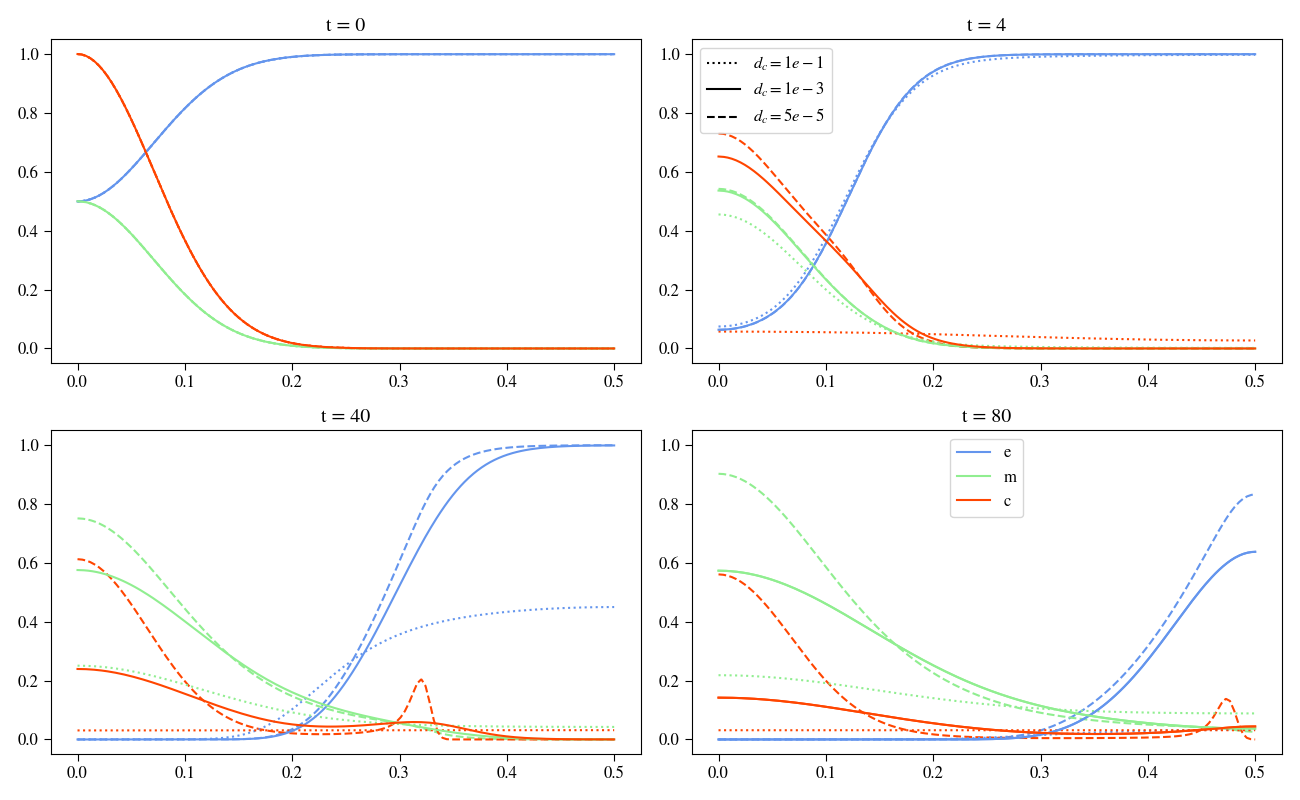
\includegraphics[width=\textwidth]{resources/images/dc_variation.png}
 \caption{Results of varying $d_c$ in the basecase parameter set, keeping the other parameters constant, using the Plot Over Line tool}
 \label{fig:dc_variation}
\end{figure}
Looking at the experiments in figure~\ref{fig:dc_variation}, we can see these assumptions met. The smaller $d_c$ gets, the higher the influence of haptotaxis; therefore, $\gamma$ will be and vice versa.

Considering the tumor cell density curves shown in red, we can see minor differences after already $t=0.4$. For the two lower values of $d_c$, the solid and dashed curves, we see the tumor cells having a higher concentration at the origin than for the biggest value of $d_c$, dotted curve, nearly overlaying each other. The red dashed curve is considerably lower at the origin, though it is stretched out more than the other two, indicating a faster invasion rate. The other curves describing EDM and MDE concentration do not show any deviations from each other at this point.

Looking at the plot results, at time $t=4$, we see the previously observed effects increase. The curves of the tumor cells confirm that with increasing $d_c$, the remaining lump of cells at the origin decreases, distributing the tumor cells more evenly in space and also reducing the effect of haptotaxis, making the secondary lump, which is still visible for the highest diffusion term, less sharp. At this point, the other two curves also show differentiating behavior. The ECM is degraded faster with increasing $d_c$ and the slope the ECM describes is less steep. Looking at the extracellular matrix, we see minor differences between the lower two values for $d_c$. Due to the tumor cells' exponential production of the MDEs and the more even spread of the tumor cells, we see them taking on a lower concentration at the origin. However, we can also observe that they have spread farther out than the MDE concentrations describing the experiments with lower $d_c$ values.

Studying the last image of $t=8$, we see no new effects, only the already mentioned propagated; with increasing $d_c$, we see a more even spread of the tumor cells and a reduction of the secondary lump, leading to the invasion of the tissue. For the MDE concentration, we observe less concentration in total due to the exponential growth rate, especially at the origin. However, we also see a more even distribution of them and a slightly faster invasion pace. This causes the extracellular matrix degradation to work faster.

Regarding the sensitivity of this parameter, the higher the value is, the more sensitive the system reacts. Though the lower two values for $d_c$ are only separated by $5\cdot 10^{-5}$ and we can unfortunately not experiment with $d_c=1 \cdot 10^{-5}$ due to numerical instabilities, the differences between those two were minimal compared to the difference between the higher two values of $d_c$.

From a biological point of view, this increase in diffusion might be caused by a change in temperature, electric potential or mechanical pressure differences. The higher diffusion results in a more even spread of the two actively moving quantities of tumor cells and matrix-degrading enzymes, which degrade their surrounding tissue, the ECM, at a faster rate.


\subsubsection*{$\gamma$ Variation}
$\gamma$ describes the effects of haptotaxis; it is assumed that it is evenly distributed in $\gamma \sim U[0.001,0.01]$, like Anderson et al. ~\cite{anderson_mathematical_2000} assumed. Like Anderson et al., we will also look at values exceeding this region, though most likely losing their biological meaning. Inspecting the effects of $\gamma$, we can assume the countering effects on the tumor cells as for varying $d_c$; selecting higher values for $\gamma$ will increase the effects of haptotaxis, creating a larger secondary lump of cells that is being pulled faster into the tissue.
\begin{figure}[h!]
 \centering
 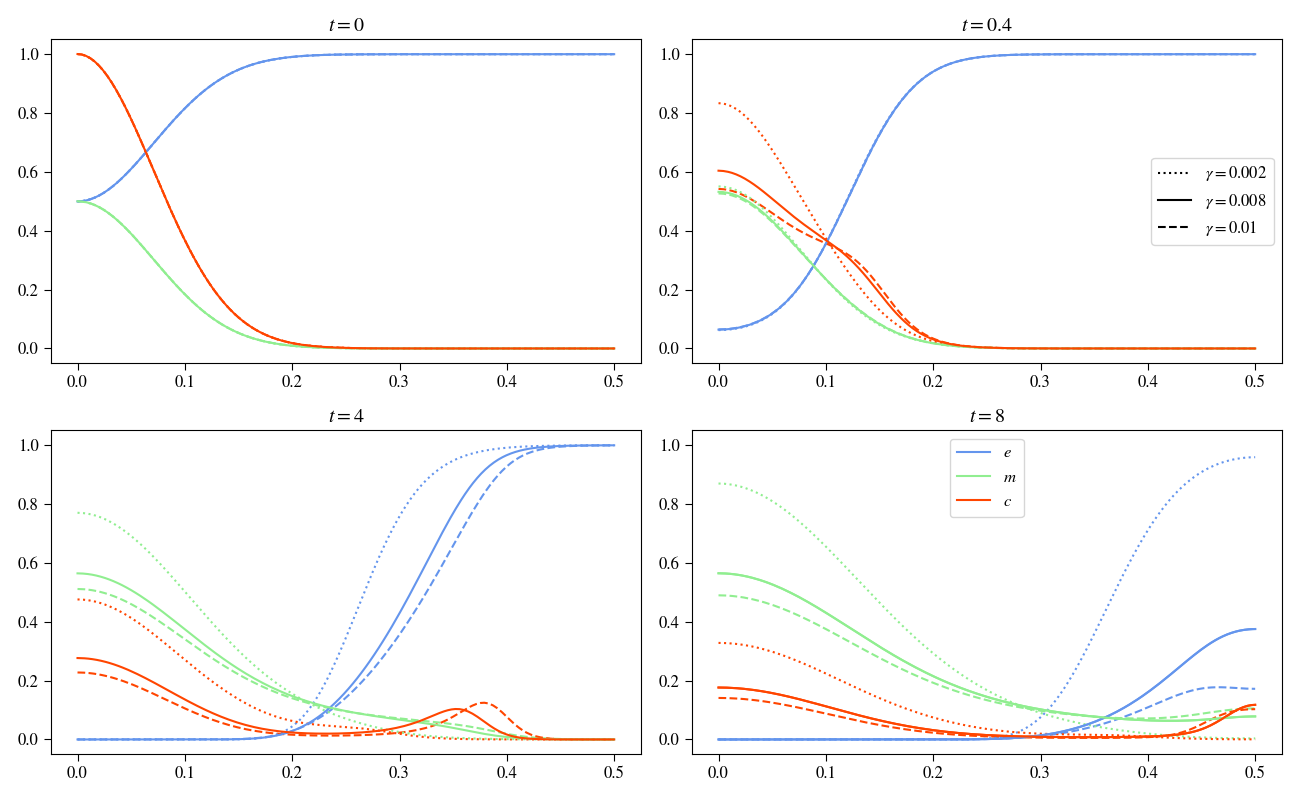
\includegraphics[width=\textwidth]{resources/images/gamma_variation.png}
 \caption{Results of varying $\gamma$ in the basecase parameter set, keeping the other parameters constant, using the Plot Over Line tool}
 \label{fig:gamma_variation}
\end{figure}
The experiments described in figure~\ref{fig:gamma_variation} verify the expected behavior.

After $t=0.4$, we already see apparent changes for varying $\gamma$; the higher $\gamma$ is set, the greater the division for the tumor cells is observable, which will later form the secondary lump. The lowest value for $\gamma$, undercutting the one for the basecase, shows no signs of a leading edge forming that invades the tissue separately. The two higher values for $\gamma$ show little deviation. Considering the other two variables, extracellular matrix concentration and matrix-degrading enzyme concentration, no change is visible, still overlaying each other at this temporal point.

The following image shows the simulation after $t=4$ timesteps; we can see changes in all three variables. 
While the tumor cell density for the values of $0.008$ and $0.01$ differ slightly by the number of cells that are left at the origin and the distance they have already invaded the surrounding tissue, the curve for the lowest $\gamma$ value, as at $t=0.4$ does not show a division of the tumor cells that invades the tissue separately, which causes the tumor cells to stay centered around $x=0$, resulting in a higher density of cells there compared to the results of the other experiments. With increasing $\gamma$, the invasion speed also increases, as the dashed line for the tumor cell density shows. For the MDE curve, we also observe that the lower $\gamma$ is, the more concentration is at the origin due to the higher remaining density of tumor cells at the origin. The ECM concentration shows behavior similar to the MDE concentration; with increasing $\gamma$, the ECM is faster and more evenly degraded; due to the faster invasion of the tissue, the production of matrix-degrading enzymes also happens in regions farther away from the center. As we saw varying $d_c$, only a little MDE concentration is needed to degrade the extracellular matrix efficiently. Therefore, the ECM degradation process also happens faster here.

In the last image at $t=8$, we see the observations from previous points in time confirmed; the higher $\gamma$, the faster the invasion pace of the tumor cells and the more of a division forms with fewer tumor cells staying at the origin. The behavior of the tumor cells causes a higher concentration of MDEs at the origin due to exponential growth and a steeper decline moving outwards. With rising $\gamma$, the ECM is getting degraded faster.

\begin{figure}[h!]
 \centering
 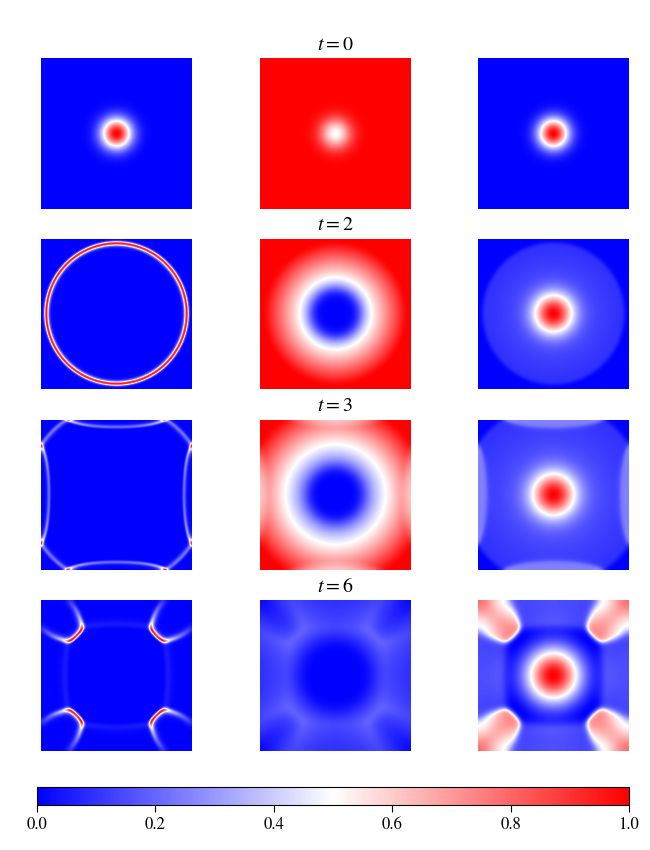
\includegraphics[width=0.95\textwidth]{resources/images/gamma_2D_plot_.png}
 \caption{2D plot showing experiment for $\gamma=0.1$, left tumor cell density, right ECM concentration}
 \label{fig:gamma_2D_plot}
\end{figure}
Out of curiosity, we will take a step further and increase $\gamma$ again by one power to $\gamma=0.1$. As previously observed, the haptotatic effects of pulling the cells into surrounding tissue increase, causing an even faster invasion pace. However, in this case, the invasion pace of the tumor cells is so high that no cells are left at the origin; everything is being pulled into the surrounding tissue. Before finishing the simulation after $t=8$, the tumor cells have reached the domain $\Omega$'s border. The cells are being reflected at the border due to the boundary conditions of our model~\ref{eq:9} and~\ref{eq:10}. In figure~\ref{fig:gamma_2D_plot}, you can see that after $t=2$, the border is reached and at $t=3$, the cells have been reflected to move into the corners, where the ECM concentration is highest. At $t=3$, the pace of the ECM degradation of the matrix-degrading enzymes has not been able to keep up with the invasion pace of the tumor cells. After being pulled into the corners at $t=3$ and degrading the ECM there, at $t=6$, the tumor cells are being pulled back toward the center of the simulation.

Though this behavior matters little from a biological perspective due to the system's boundary conditions reflecting the movement and high invasion pace of the tumor cells, it is still interesting to investigate this case from a numerical perspective.

Though the intuition is met that with increasing $\gamma$, the invasion pace of the tumor cells and matrix-degrading enzymes also rises, we get unexpected behavior in the last experiment. There is more of a total ECM concentration left than in the experiment using $\gamma=0.01$.
Studying those experiments biologically, we know that the term extracellular matrix describes a whole class of different molecules, minerals or proteins, like collagens or enzymes. The different properties of these elements cause varying effects of haptotaxis. For example, were the haptotatic effects measured on laminin considerably lower than then ones measured on fibronectin, according to Aznavoorian et al.~\cite{article}. Different constellations of extracellular matrix composition will be encountered in different human body sites, which will cause the tumor cells, as seen in the numerical experiments, to behave differently.

\subsubsection*{$\eta$ Variation}
The parameter $\eta$ controls the degradation process of the extracellular matrix molecules. Since Anderson et al.~\cite{anderson_mathematical_2000} used a value of $\eta=10$ on all their experiments, we assumed an even distribution in $\eta \sim U[0, 20]$. The degradation process of the extracellular matrix is modeled using an exponential decay hypothesis, so we can expect that increasing $\eta$ also increases the system's sensitivity concerning the parameter $\eta$. With its role in controlling the degradation, it will also heavily influence the motility of the tumor cells and, therefore, the motility and production rate of the matrix-degrading enzymes. Slower degradation will result in a higher density of tumor cells at the origin, exponentially producing matrix-degrading enzymes. This, in turn, will increase the ECM degradation. With increasing $\eta$, the ECM is faster degraded and, therefore, might provoke a faster invasion rate of the tumor cells of the surrounding tissue. The higher $\eta$ is, the fewer MDEs are needed to degrade the ECM efficiently.

\begin{figure}[h!]
 \centering
 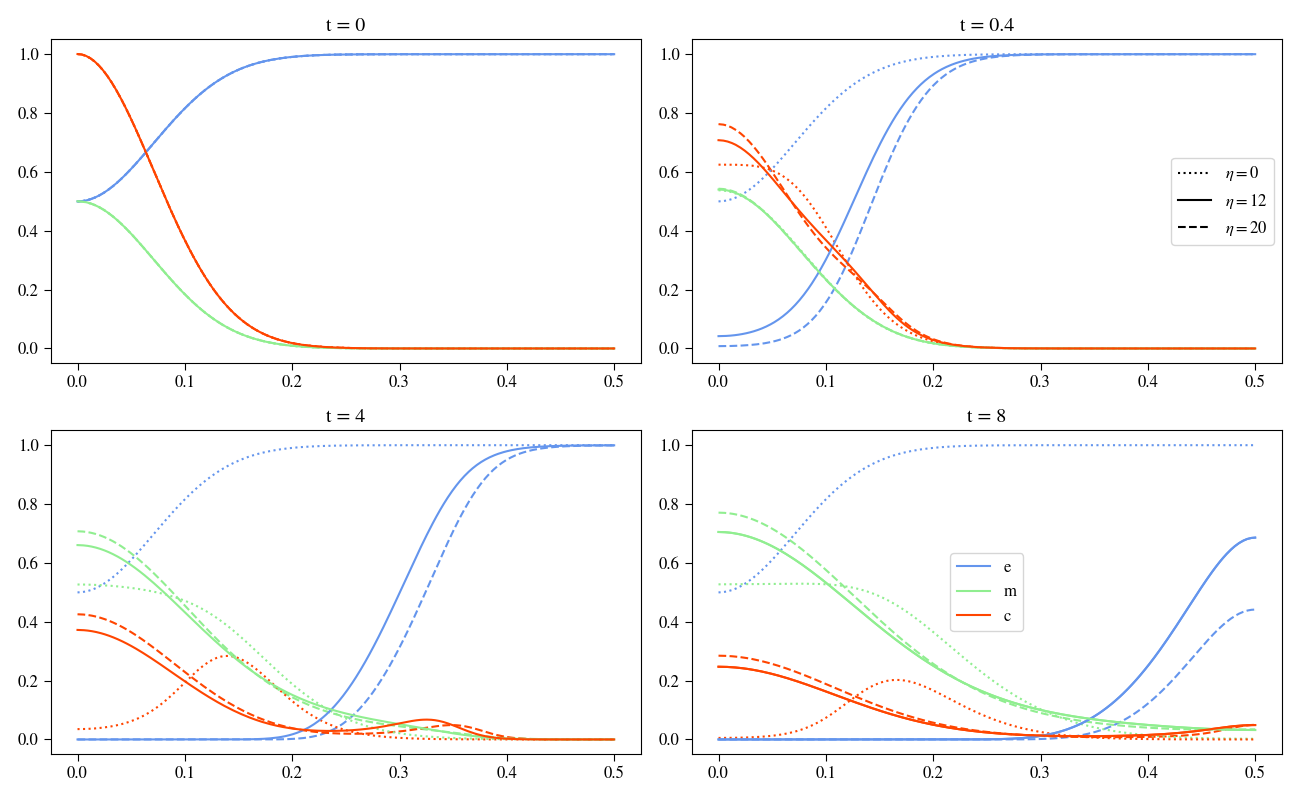
\includegraphics[width=\textwidth]{resources/images/eta_variation.png}
 \caption{Plots show results for varying $\eta$ while keeping the other parameters constant; in the images you can see the effects of $\eta=20$ in the dashed curve, $\eta=0$ in the dotted curve and $\eta=12$ in the solid line.}
 \label{fig:eta_variation}
\end{figure}
Inspecting the results in figure~\ref{fig:eta_variation}, it is most striking that the slower degradation rate causes a slower tumor invasion. 

We see significant differences for both curves, tumor cell density and ECM concentration after $t=4$. Inspecting the experiment with $\eta=2$, we see that the ECM has only degraded a little, exposing the tumor cells to stronger haptotatic pull by the ECM in regions closer to zero, compared to the other experiments. Though it may look like no secondary lump of cells is being formed, the contrary is the case; even more cells are pulled into the tissue, with the ECM slowly receding into the tissue, which smoothes out the bump the other two curves show for the tumor cell density. This results in only one lump of tumor cells that invades the tissue without one remaining at the origin. The same effect is observable when comparing the tumor cell density curves for the higher $\eta$ values. With fewer tumor cells pulled by the ECM, the higher $\eta$ gets. Only the curve for the matrix-degrading enzymes has not been affected by the variation of $\eta$ until now.

The next image at $t=4$ propagates the effects on the tumor cells and the ECM. The slower the degradation process, the more tumor cells invade the tissue and the less of a division is observable. The movement now also affects the concentration of the matrix-degrading enzymes. With the fewer remaining tumor cells at the origin producing the MDEs, we also see a more minor concentration at the origin. However, the distribution of the tumor cells for the lowest case of varying $\eta$ has a more even distribution of MDEs.

The same goes for the last image, showing the experiments at $t=8$. The more even the distribution of tumor cells and matrix-degrading enzymes across space, the slower the ECM is degraded.

As mentioned, varying $\gamma$ does the term extracellular matrix include various organic or inorganic compounds. Therefore, the build-up and properties of these compounds vary strongly and motivate this comparison of degradation rate. Some compounds may be degraded faster, while others are complex and need more time to degrade. 

\subsubsection*{$d_m$ Variation}
$d_m$ describes the diffusion coefficient for the matrix-degrading enzymes. As estimates, we use Anderson et al.'s and Franssen et al.'s values, which assume an even distribution of $d_m$ in $\sim U[1\cdot 10^{-5},1\cdot 10^{-3}]$. Having set $\beta=0$, equation~\ref{eq:8} modeling the temporal development of the matrix-degrading enzymes concentration only depends on c concerning motility as well as in production. As we saw in experiments before, we can expect a high concentration of MDEs in regions with a high density of tumor cells and we can expect increased motility where the density of the tumor cells rapidly changes. Increasing $d_m$ will cause a faster, more even spread of the MDEs in the surrounding area and therefore, the ECM will also be degraded faster.

\begin{figure}[h]
 \centering
 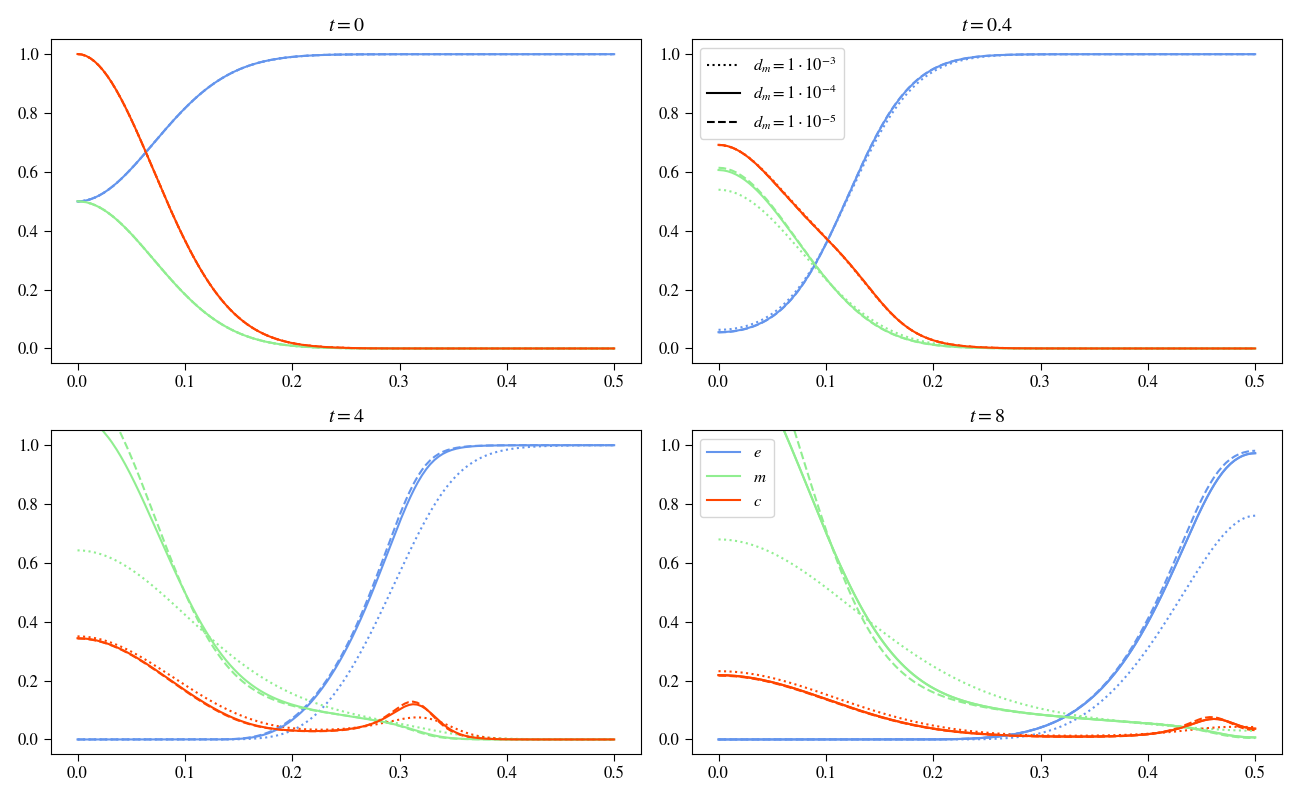
\includegraphics[width=\textwidth]{resources/images/dm_variation.png}
 \caption{Plots show results for varying $d_m$ while keeping the other parameters constant; in the images you can see the effects of $d_m=0.1$ in the dashed curve, $d_m=0$ in the dotted curve and $d_m=1\cdot 10^{-3}$ in the solid line.}
 \label{fig:dm_variation}
\end{figure}
Inspecting the results in figure~\ref{fig:dm_variation}, we observe that in the second image after $t=0.4$, the curves of the tumor cell density and the ECM are mostly untouched, though looking closely, we can see that for the highest $d_m$ value, dotted line, the ECM has at the origin higher and farther out lower concentrations of the ECM. This is caused by the more even distribution of the matrix-degrading enzymes, which visibly reduce the concentration at the origin and invade the surrounding tissue slightly faster at this point.

The following image shows the experiments after $t=4$ and we see the differences between the lowest $d_m$ value experiment with the other two more pregnant. The MDE concentration has, relative to the other two, strongly decreased at the origin, though it has invaded the tissue further. The ECM has degraded faster and as we saw in the $\eta$ variation, the faster ECM degradation reduces the effects of haptotaxis. The other two experiments differ only visibly regarding the MDE concentration, though it exceeds the limits of the plot. The concentration at the origin for the lowest diffusive value is considerably higher than for the middle value.

The last image confirms the above mentioned effects, with the most substantial deviations between the highest $d_m$ experiment and the other two. Again, a more even spread of the MDEs with a lower concentration at the origin, a faster ECM degradation and tumor cell density curves that, compared to the other experiments, have less of a division at its leading edge. The two experiments with lower $d_m$ values still have nearly overlaying tumor cell density and ECM curves. Only the MDE concentration differs between the two, showing a more even spread for the higher diffusion value, though with a lower value at the origin. 

Seeing those effects, we saw our intuition met, though it is to say that looking at the lower two values for $d_m$, the differences here were modest. Therefore, the higher the value for $d_m$ is, the more sensitive the system reacts to this change.

These changes in diffusion, like in the section varying the diffusion coefficient of the tumor cells, might be caused by a multitude of physical influences, such as temperature, voltage, pressure, etc. The results show that this change causes a faster degradation of the extracellular matrix molecules but a less aggressive invasion of the tumor cells. 

\subsubsection*{$\alpha$ Variation}
The parameter $\alpha$ influences how fast the tumor cells produce matrix-degrading enzymes. We assume it to be evenly distributed with $\alpha \sim U[0, 1.0]$ since Anderson et al. assumed the same range in the original paper. Trying to replicate Anderson et al.'s experiment, we already saw how varying $\alpha$ affects the simulation results. With growing $\alpha$, we will see a higher concentration of MDEs, especially in regions with high tumor cell density. More MDEs will cause faster degradation of the ECM first due to having more of them, but also because since more of them are subject to diffusion, they will spread faster in the tissue. Faster ECM degrading could mean an increased invasion pace of the tumor cells. As we saw in the previous experiments varying $d_c$, the MDE concentration can take on values higher than one. We can also expect this here when $\alpha$ is sufficiently high. 
\begin{figure}[h]
 \centering
 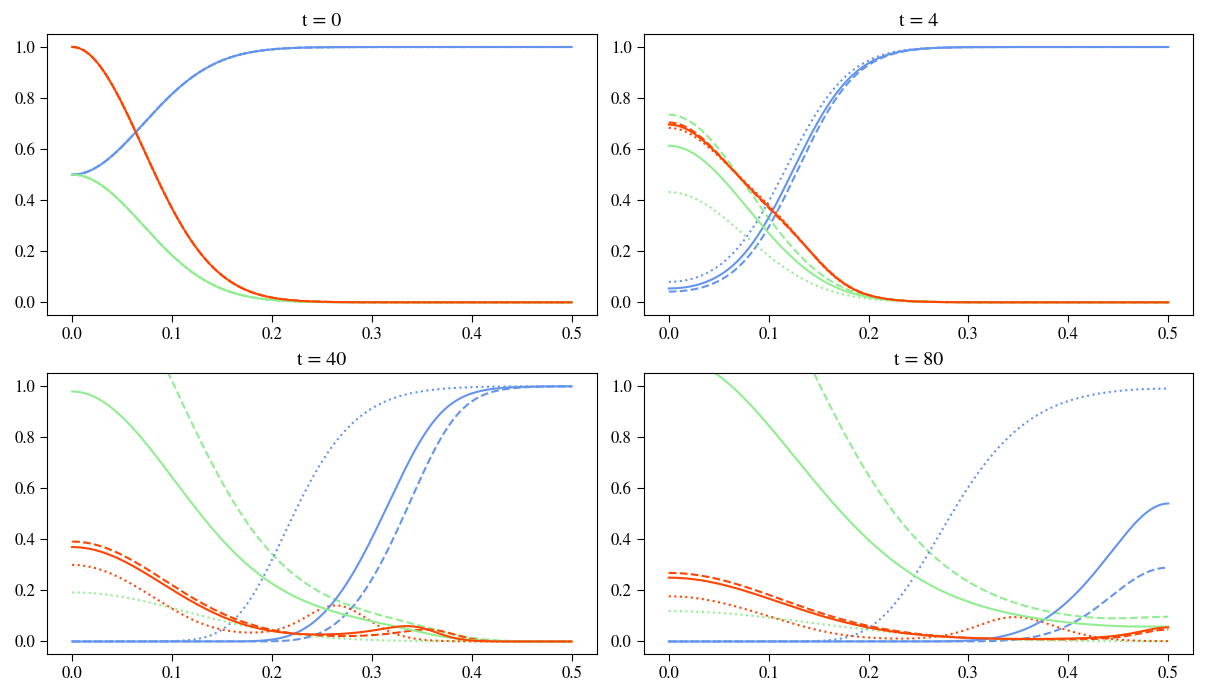
\includegraphics[width=\textwidth]{resources/images/alpha_variation.png}
 \caption{Plots show results for varying $\alpha$ while keeping the other parameters constant; in the images, you can see the effects of $\alpha=1.0$ in the dashed curve, $\alpha=0$ in the dotted curve and $\alpha=0.6$ in the solid line.}
 \label{fig:alpha_variation}
\end{figure}

The second image of figure~\ref{fig:alpha_variation} describes the experiments after $t=0.4$. We can clearly see the differences in the MDE curves for the different values of $\alpha$. The other curves also show slight deviations. The higher $\alpha$ is, the faster the ECM degradation. Looking closely, we can observe for the tumor cell density that the increased rate of ECM degradation results, as previously already seen, in a curve with less of a bump that will later form the division invading the surrounding tissue due to more minor haptotatic influences at the origin.

The next point in time, at $t=4$, shows the previously mentioned effects in a reinforced way. For $\alpha=0$, the MDEs have no producing factor and the curve flattens due to diffusion, though the extracellular matrix has degraded visibly, yet at a considerably slower rate. This experiment has the lowest density of tumor cells at the origin, though the most significant secondary lump of cells invades the tissue. This behavior is due to the extended exposition of strong haptotatic influences near the origin region, which pulls more cells outward to invade.
The solid curves describing $\alpha = 0.6$ show that at this point, they have almost reached a concentration of one at the center, which will be exceeded later. Compared to the lowest $\alpha$ experiment, the faster ECM concentration has also pulled less of the tumor cells outward, though at a faster invasion pace. 
Looking at the experiment with the highest $\alpha$ value, the MDE concentration already exceeds one, the ECM degradation is happening faster and the invasion of the tumor cells is happening faster, though with a lower density.

In the last timestep, we see that the MDE curve of $\alpha=0.6$ and $\alpha=1.0$ exceeded one. For the dotted curve of the MDE, we have a good example of diffusion distributing the concentration throughout space without changing its overall volume. At the border regions, we see that the dotted curve is also the only one that has yet to degrade any ECM in this area, while the other two experiments show that there is only a little ECM concentration left to degrade. 
The tumor cells confirm the, in the previous timestep mentioned, effects of faster invasion pace with rising $\alpha$ though with at a thinner density.


Our initial assumptions were correct with a faster degradation pace due to higher MDE concentration and, therefore, a faster invasion pace of the tumor cells. However, it is interesting to see that the more minor $\alpha$, the more tumor cells are being pulled into the tissue.

While it makes sense from a numerical perspective that the concentration of MDEs can exceed one, it might make sense to introduce a finer grid or adapt the model in other ways since, judging from a continuous perspective, it does not make sense that at a certain point in space, there is more than one entity occupying this space.

The production of matrix-degrading enzymes can have many biological causes. During many natural processes like tissue repair or remodeling, the extracellular matrix must be degraded, controlled by cells producing enzymes that, in turn, are responsible for producing matrix-degrading enzymes. This control flow can be interrupted by malignant cells stimulating the production of MDEs without any repair or remodeling tasks to perform. Considering the absence of or reduced MDE production, we can regard this case as the consequence of a drug treatment. On the other hand, since there are plenty of different extracellular matrix molecules, they may also have different production rates.


\subsubsection*{$\beta$ Variation}
The factor $\beta$ controls the decay of the matrix-degrading enzymes and the results of its variation are shown in figure~\ref{fig:beta_variation}. Using Kolev et al.'s estimate for $\beta$ in \cite{Kolev2010}, we experimented with $\beta=0.07$. Considering the results, we can assume an even distribution of $\beta$ in $\beta \sim U[0.005, 0.1]$. Interestingly, $\alpha$ and $\beta$ are their respective distribution and the experiments will confirm that they are not of the same magnitude. While the MDEs are produced by the tumor cells, their decay is controlled by the MDEs themselves. This model assumes that the tumor cells do not proliferate, which makes their total amount constant. In contrast, the MDEs are produced by the tumor cells and are expected to change in amount over time due to production or decay. This makes the decay rate of the MDEs more variable because of the changing amount of total MDEs, causing the change of effective magnitude.

With introducing $\beta$ foremost, we can assume that the MDE curve will be lower, influencing the ECM degrading process and, therefore, the invasion pace and the diffusion-haptotaxis effects on the tumor cells. 

\begin{figure}[h]
 \centering
 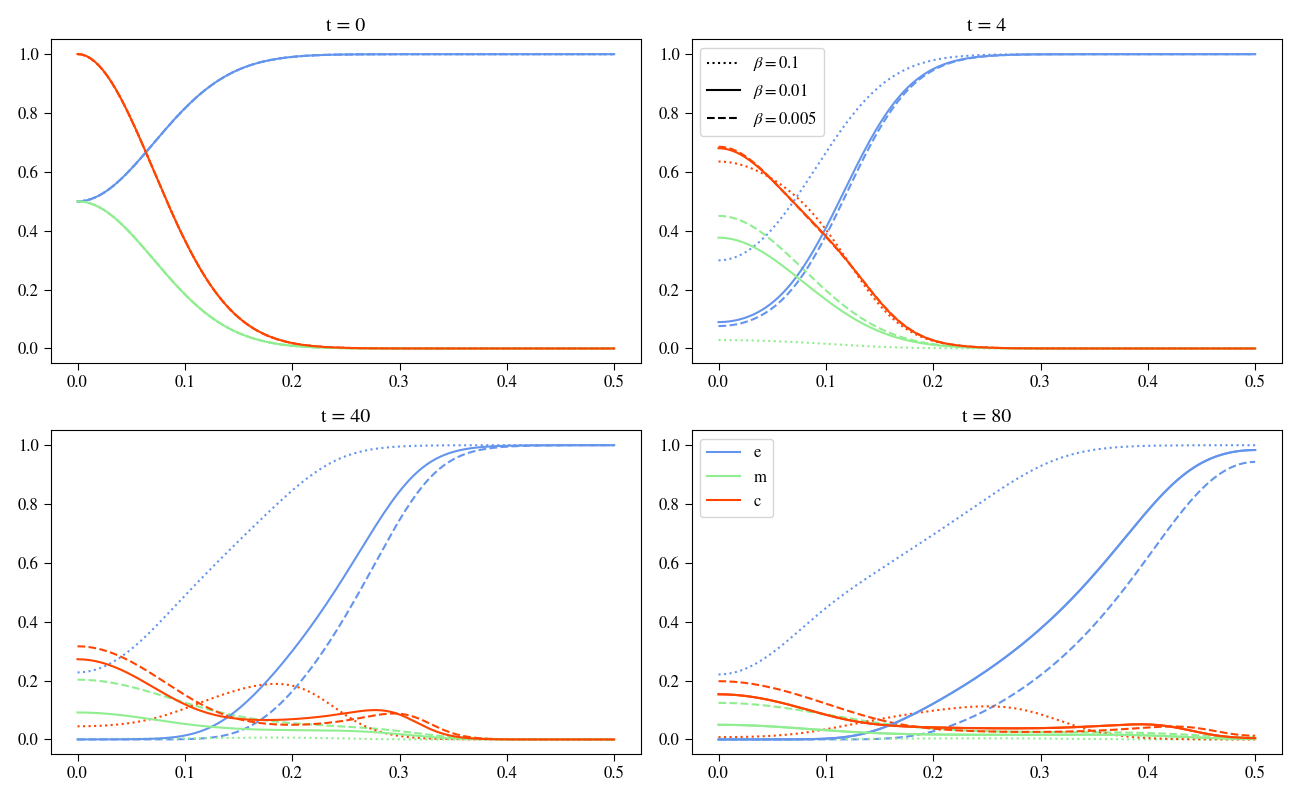
\includegraphics[width=\textwidth]{resources/images/beta_variation.png}
 \caption{Plots show results for varying $\beta$ while keeping the other parameters constant; in the images, you can see the effects of $\beta=0.005$ in the dashed curve, $\beta=0.1$ in the dotted curve and $\beta=0.01$ in the solid line.}
 \label{fig:beta_variation}
\end{figure}
As we see from the results in figure~\ref{fig:beta_variation}, a value of $\beta=0.1$ is sufficient to after already $t=4$ reduce the MDE concentration to nearly zero. In our case, this decay rate proves too high, outpacing production entirely, with matrix-degrading enzyme concentration vanishing spacially and temporarily completely. The immediate decay of the MDEs causes a drastically slower ECM degradation, yet it has not stopped entirely since the tumor cells still produce matrix-degrading enzymes. This slow degradation of the extracellular matrix, as we saw previously, creates a haptotatic pull that lasts a lot longer in regions around the origin, which pulls, in this case, all of the cells outward to invade the tissue, leaving no primary lump of tumor cells at the origin. Since more MDEs are produced in regions with high tumor cell density, this also causes a more even degradation of the extracellular matrix, causing a more substantial stretch of the tumor cells.

In the other experiments, we can observe that with decreasing $\beta$ and slowing down the decay of the matrix-degrading enzymes, first, the ECM degradation accelerates and this causes the effects of haptotaxis and diffusion to develop the two lumps of tumor cells, one staying at the center the other invading the tissue as we saw in all previous experiments.

Since the extracellular matrix can comprise many different organic and inorganic compounds, the degrading enzymes are also very diverse. This diversity results in different decay rates, so choosing the right one for a specific experiment can be crucial. While this variation describes the effects of different enzymes, it can also describe, like for the production of the MDEs, the influence of a drug to accelerate the decay of the matrix-degrading enzymes.

\subsubsection*{Cross-Variation}
Having varied every model parameter, we saw accelerating effects on the invasion and countering effects. Now, it will be interesting to see how either supporting factors interplay and how countering factors affect the simulations, for example, how to increase both $\alpha$ and $\beta$ if some balance can be found. Another exciting experiment will be on how diffusion and haptotaxis behave when increasing or decreasing both factors controlling them.

\subsubsection*{$d_c - \gamma$ Variation}
\begin{figure}[h!]
 \centering
 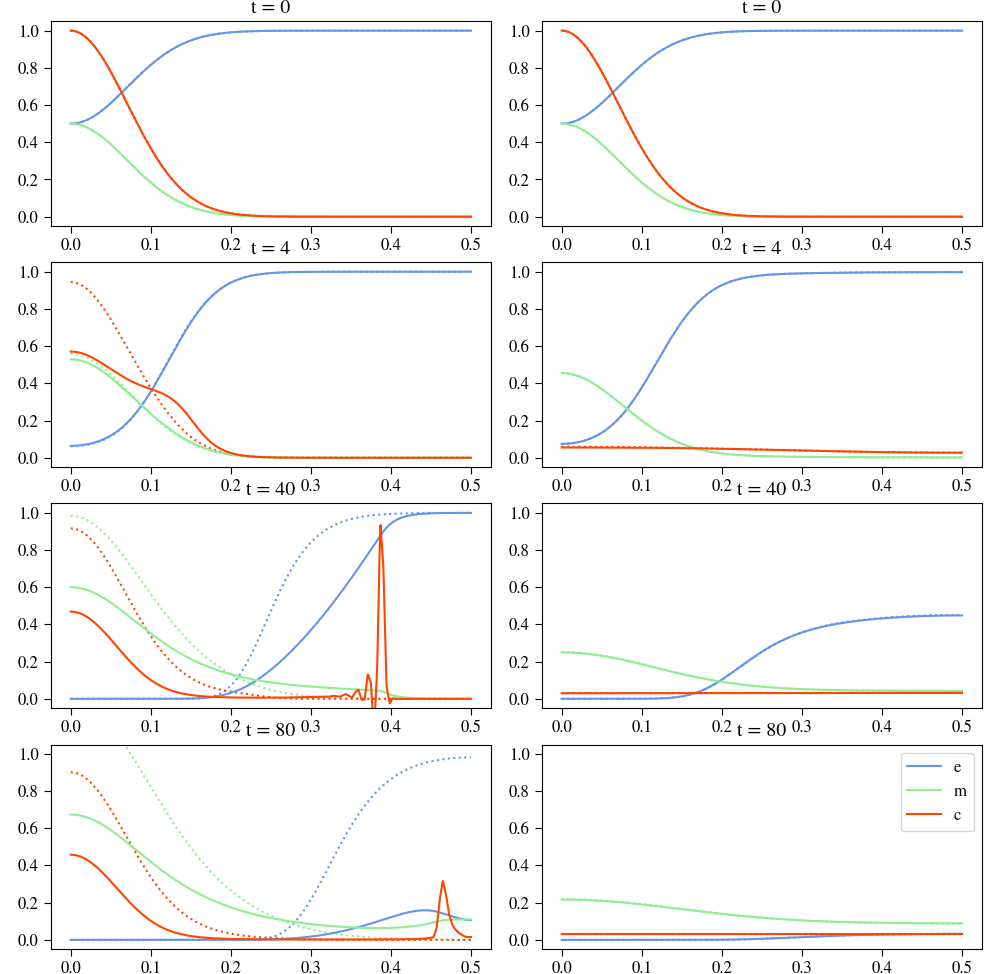
\includegraphics[width=\textwidth]{resources/images/dc_gamma_variation.png}
 \caption{Plots show results for varying both $d_c$ and $\gamma$ while keeping the other parameters constant; in the images on the left, $d_c$ is set to $d_c=0.00005$ with the solid line showing $\gamma = 0.01$ and the dotted line $\gamma=0.001$ on the right $d_c$ is set to $d_c=0.1$ with the solid line showing $\gamma = 0.01$ and the dotted line $\gamma=0.001$.}
 \label{fig:dc_gamma_variation}
\end{figure}
We, therefore, started with varying $d_c$ and $\gamma$ and studied for simplicity and overview reasons only the values on their distribution's borders interplaying, shown in figure~\ref{fig:dc_gamma_variation}.

Having set $d_c=5\cdot 10^{-5}$ and $\gamma=0.001$, we see no division of the tumor cells; the effects of haptotaxis are too small, leaving the tumor cells only subject to diffusion, which results in an even distribution process over time, which also causes a slower invasion pace. Because the tumor cells stay in a lump with their maxima at the origin $x=0$, the MDEs also take on their maximum there, moving farther out and distributing very evenly. This staying with values around the origin of the MDEs causes a slower ECM degradation. 

Increasing $\gamma=0.01$, we see that the effects of haptotaxis are now pregnantly visible with a very sharp maximum seen at $t=4$, which equals the maxima of the remaining tumor cell lump at $x=0$. A more substantial influence of haptotaxis leads to a faster invasion pace of the tumor cells into the tissue. It allows the creation of matrix-degrading enzymes in their wake, causing a more even distribution compared to $\gamma=0.001$ and a faster ECM degrading process. 

Looking at the right side of the plot~\ref{fig:dc_gamma_variation}, we see the results for $d_c=1 \cdot 10^{-3}$. Comparing $\gamma$ values with this $d_c$ value, we can, as on the left side, see that the experiment showing $\gamma=0.001$ does not form a division for the tumor cells, with the main lump of cell staying at the origin. No secondary site of tumor cells is formed that invades the tissue faster. This is also shown on the ECM concentration for the dotted experiment, with a considerably slower degradation process and when comparing both dotted experiments on left and right side images. Staying near the center of the tumor cells also causes a much higher MDE concentration there compared to the $\gamma$-increased experiment. 

Increasing both $d_c$ and $\gamma$, we see the effects of haptotaxis more potent with the secondary site of tumor forming. However, comparing this experiment with the experiment having high $\gamma$ and low $d_c$ values shows that the division has no peaky leading edge.

These experiments give us an excellent example of the relationship between haptotaxis and diffusion. We see that with decreasing $d_c$ but increasing $\gamma$, we get a leading edge that is very pointy. The higher value of $\gamma$ was sufficient to form a secondary tumor site invading the tissue separately. Decreasing $\gamma$ has proven for high and low $d_c$ values to prevent a secondary lump of cells from forming. 

\subsubsection*{$d_m - \eta$ Variation}
\begin{figure}[h!]
 \centering
 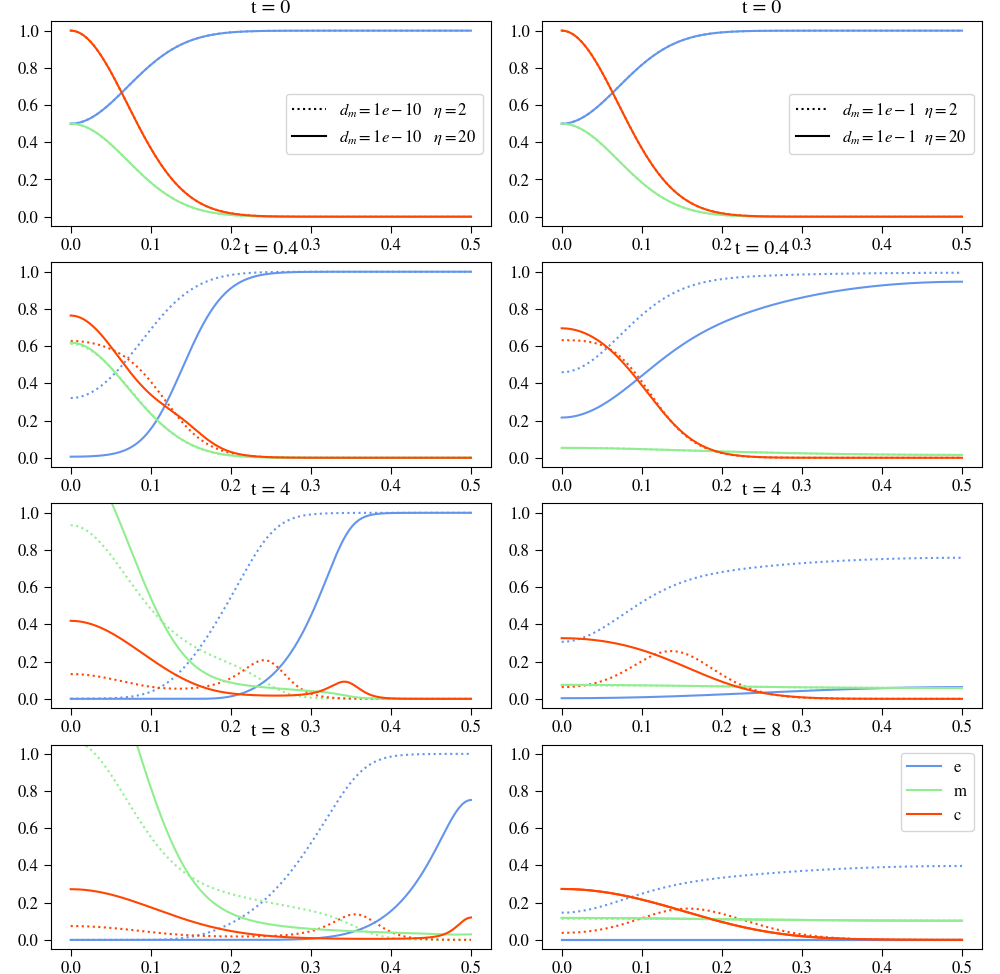
\includegraphics[width=\textwidth]{resources/images/dm_eta_variation.png}
 \caption{Plots show results for varying both $d_m$ and $\eta$ while keeping the other parameters constant, in the images on the left $d_m$ is set to $d_m=1\cdot 10^{-5}$ with the solid line showing $\eta = 2$ and the dotted line $\eta=20$ on the right $d_m$ is set to $d_m=1\cdot 10^{-3}$ with the solid line showing $\eta = 2$ and the dotted line $\eta=20$.}
 \label{fig:dm_eta_variation}
\end{figure}

Comparing both columns for varying $d_m$ in figure~\ref{fig:dm_eta_variation}, though looking at the same $\eta$ valued experiments, we can only see minor differences regarding the shape of the tumor cell density curve and ECM concentration curve. On the left side, we see that the ECM degradation is happening slower, which causes a different relation regarding the diffusion-haptotaxis effects. The curves on the left side are not as evenly stretched as on the right, with a more significant hill at the secondary lump of cells. This behavior is due to the extended exposition of more substantial haptotaxis effects on the tumor cells in regions closer to the origin. 

The ECM degradation is happening slower on the left side due to minor diffusive motility, which is slowing the MDE invasion process.

Interestingly, the MDE concentration for lower $d_m$ values is considerably higher for both experiments than for the ones with higher $d_m$ values. Since the tumor cells produce the MDEs, it is apparent that only the slightest visible change in the tumor cell density is sufficient to cause such drastic changes in the production of the MDEs due to exponential growth. 

These experiments conclude that the diffusive properties of the matrix-degrading enzymes play only a minor role in degrading the extracellular matrix. Tumor cells producing them in their wake play a more crucial role in the degradation process. An intriguing observation in this experiment is that minimal differences in tumor cell density are sufficient to create major differences in the MDE concentration due to their exponential production.

\subsubsection*{$\alpha - \beta$ Variation}
\begin{figure}[h!]
    \centering
    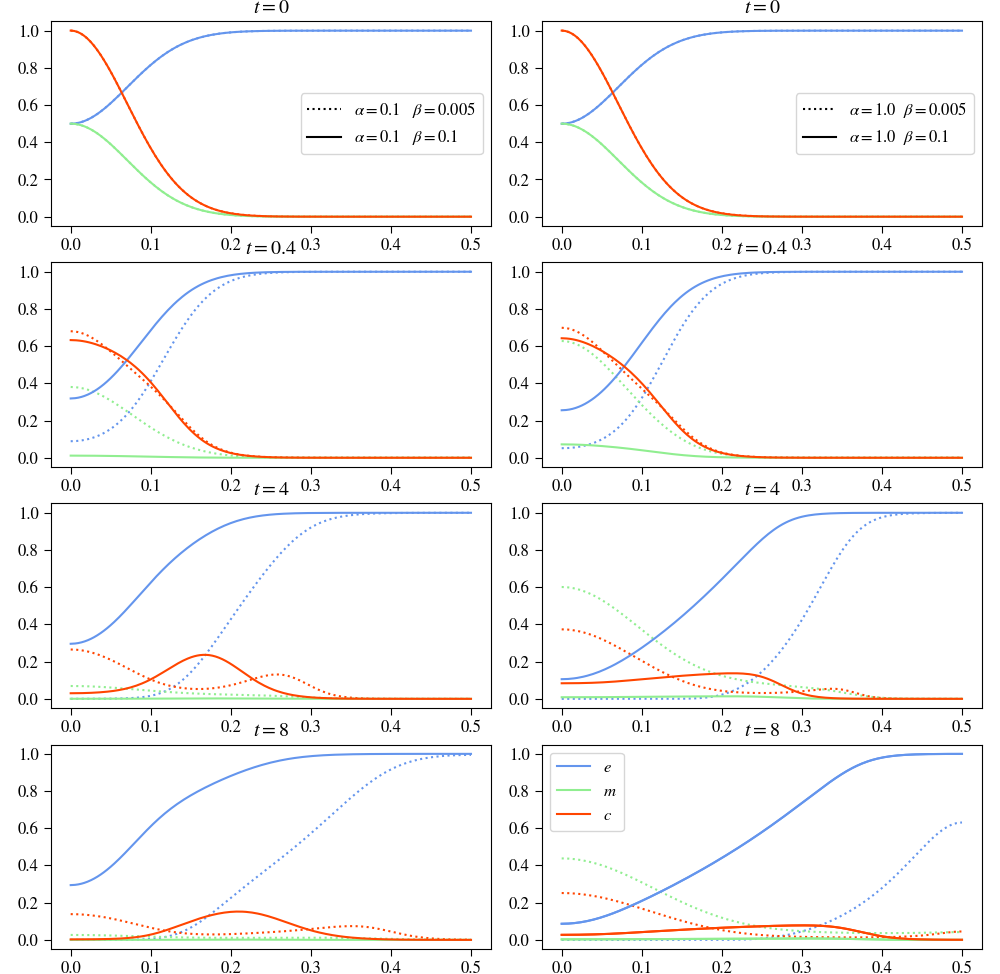
\includegraphics[width=\textwidth]{resources/images/alpha_beta_variation.png}
    \caption{Plots show results for varying both $\alpha$ and $\beta$ whilst keeping the other parameters constant, in the images on the left $\alpha=0.1$ with the solid line showing $\beta = 0.005$ and the dotted line $\beta=0.1$ on the right $\alpha=1.0$ with the solid line showing $\beta = 0.005$ and the dotted line $\beta=0.1$.}
    \label{fig:alpha_beta_variation}
\end{figure}


Looking at figure~\ref{fig:alpha_beta_variation} we see experimental results varying both $\alpha$ and $\beta$. For low MDE production and low MDE decay, we can see that the curve for the MDEs is still visible at up to $t=4$; at $t=8$, it is zero. We see that the ECM degrading happens faster than for high $\beta$ values; therefore, the tumor cells develop two lumps, with one invading the tissue and the other staying at $x=0$. The maxima for both lumps are lower than in previous experiments, though the cells seem to be more evenly distributed between the two lumps. Increasing $\beta=0.1$, the MDE curve appears to be zero after already $t=0.4$ and stays there until the end of this experiment. This low concentration of MDEs causes a slower ECM degrading process, leading the tumor cells to develop only one lump, invading the space, with its maxima moving at the center of this lump. For $\alpha=0.1$, both values for $\beta$ have proven too high, decaying the matrix-degrading enzymes too fast to keep up with production.

On the other hand, increasing $\alpha$ to $1.0$ and keeping $\beta=0.05$, we see that production outweighs decay, with at the end of the experiment, the MDEs still have a concentration of about $0.4$ at $x=0$. For this experiment, we see that the tumor cells develop two lumps, indicating that diffusion and haptotaxis effects are also in some balance and ECM degradation seems to resemble, due to similarities with the basecase for the MDE curve, also the ECM degradation of the basecase experiment.
Increasing both $\alpha$ and $\beta$, we see in the solid line of the right column of figure~\ref{fig:alpha_beta_variation} that decay outweighs production again, after $t=0.4$ we can only see a small remaining portion of matrix-degrading enzymes at the origin. This causes slower ECM degradation and forms only one lump of tumor cells due to the strong effects of haptotaxis, though this singular lump is stretched flat along the x-axis.

\subsubsection*{$d_m - \alpha - \beta$ Variation}
\begin{figure}[h!]
    \centering
    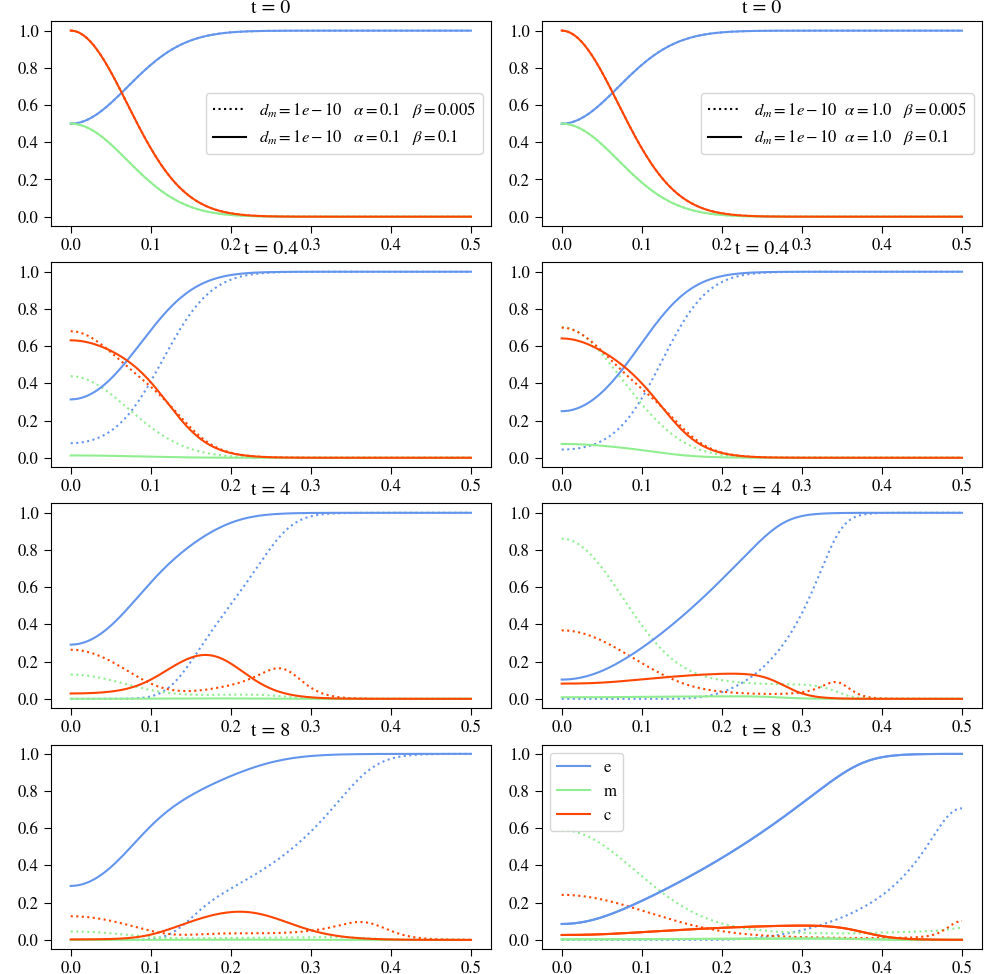
\includegraphics[width=\textwidth]{resources/images/dm_alpha_beta_variation_1.png}
    \caption{Plots show results for varying both $\alpha$ and $\beta$ whilst keeping the other parameters constant, in the images on the left $\alpha=0.1$ with the solid line showing $\beta = 0.005$ and the dotted line $\beta=0.1$ on the right $\alpha=1.0$ with the solid line showing $\beta = 0.005$ and the dotted line $\beta=0.1$.}
    \label{fig:dm_alpha_beta_variation_1}
\end{figure}
\begin{figure}[h!]
    \centering
    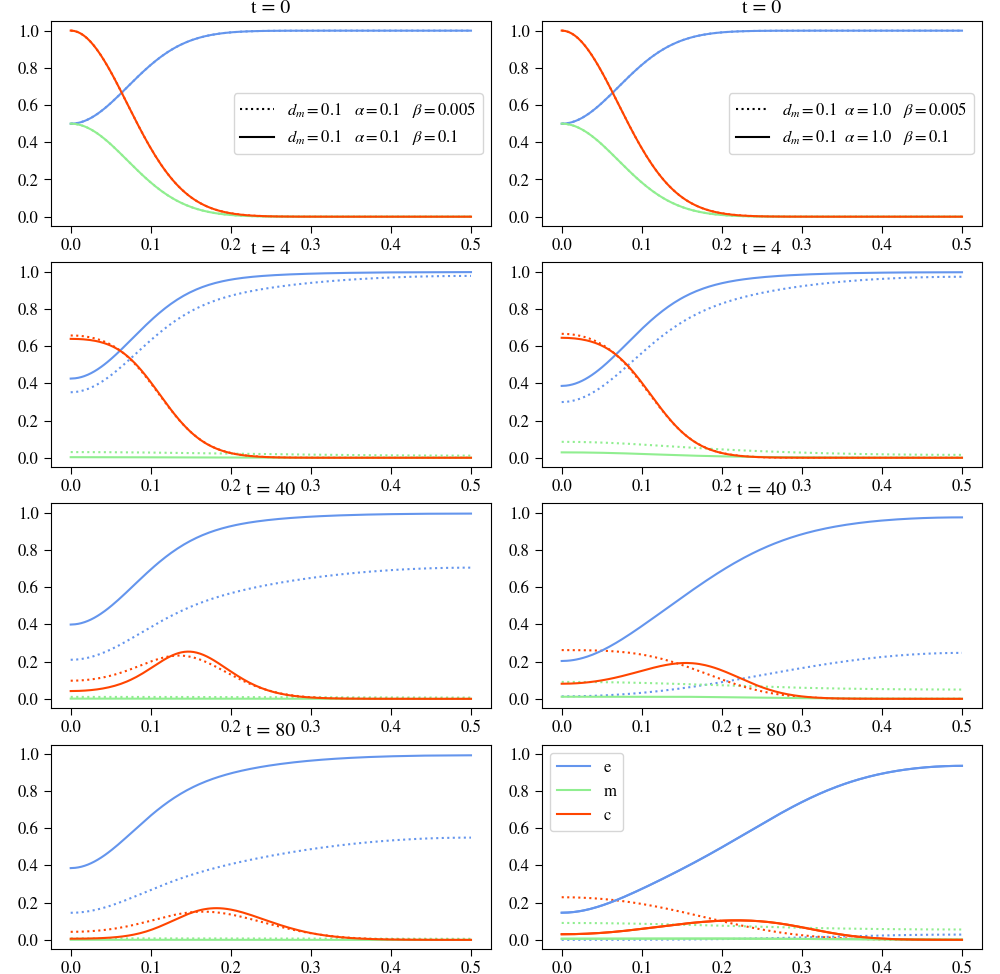
\includegraphics[width=\textwidth]{resources/images/dm_alpha_beta_variation_2.png}
    \caption{Plots show results for varying both $\alpha$ and $\beta$ whilst keeping the other parameters constant, in the images on the left $\alpha=0.1$ with the solid line showing $\beta = 0.005$ and the dotted line $\beta=0.1$ on the right $\alpha=1.0$ with the solid line showing $\beta = 0.005$ and the dotted line $\beta=0.1$.}
    \label{fig:dm_alpha_beta_variation_2}
\end{figure}

Varying all parameters regarding the equation for the matrix-degrading enzymes required to split the results into two figures,~\ref{fig:dm_alpha_beta_variation_1} and ~\ref{fig:dm_alpha_beta_variation_2}.

Looking at the results, we see that for the same $\alpha$ and $\beta$ values, the curve describing the tumor cell density shares the behavior across varying $d_m$. For low $\beta$ values, we see in every experiment that the tumor cells develop the secondary lump that detaches from the primary lump and invades the surrounding tissue separately. Considering how $\alpha$ influences this lump, we observe that with increasing $\alpha$, the lump gets smaller and more of the tumor cells stay near the origin. Taking the experiments with high $\beta$ values in regard, we observe that this curve fails to develop a secondary lump of tumor cells to invade separately. As seen in all the experiments varying $\eta$, a slowed degradation rate of the extracellular matrix leads to the extended exposition of the tumor cells at the origin to more substantial haptotaxis effects. This leads to all tumor cells being pulled outward, leaving little or no near the origin. This results in only one lump of cells that invades, with its maximum moving into the surrounding tissue. In the experiments with high values for $\beta$, we see that the diffusion of the matrix-degrading enzymes has nearly no effect, as there are no apparent changes in the plot images.

Taking the curve of the extracellular matrix into account now, we can also see minimal deviation when varying $d_m$. We see no apparent changes in figures~\ref{fig:dm_alpha_beta_variation_1} and~\ref{fig:dm_alpha_beta_variation_2} regarding the ECM concentration which supports our claim from above that the diffusion of the matrix-degrading enzymes plays only a minor role in degrading the ECM, but also for the whole system in total.

The MDE curve can explain the effects mentioned above on ECM and tumor cell density curves. We see that for every experiment where $\beta$ was set to $\beta=0.1$, the curve of the MDEs was after already $t=0.4$ zero. Increasing the production rate $\alpha$ was visibly insufficient to counter the matrix-degrading enzymes' fast decay process, resulting in the drastically slowed ECM degradation process, which in turn is responsible for the haptotaxis effects on the tumor cells. This explains why we saw no visible changes in the experiments varying $d_m$ and $\alpha$. This again shows the significance of the decay parameter of the matrix-degrading enzymes. 


\subsection{2D Results with Proliferation and Renewal - Homogenous ECM}
This section will examine how introducing tumor cell proliferation and extracellular matrix renewal influences the system. Modeled as logistical growth terms, with a limiting factor of spacial occupation, the parameters $\mu_1$ for tumor cell proliferation and $\mu_2$ for extracellular matrix renewal describe their influences. Those parameters were also incorporated in the previous experiments, though they were set to zero. Instead of treating them as parameters to vary, we are inspecting the whole system as new since they can drastically change the resulting simulations.

Tumor cell proliferation describes the natural ability of cells to proliferate. However, in the case of tumor cells, the production signaling comes from themselves, surpassing the control chain that limits normal cells to proliferate uncontrollably.

The extracellular matrix is a naturally dynamic structure that undergoes continuous degradation and remodeling. It does this in order to secure tissue development, wound repair tasks, regulate cellular functions and many more tasks. In a model describing the ECM, it is crucial to introduce a factor that incorporates these remodeling processes.

As in section~\ref{sec:2D_without_proliferation}, we use the same initial conditions for all three variables, assuming we have a homogenous ECM structure. Figure~\ref{fig:2D_homogenous_ECM_initial} depicts these initial conditions on the three variables $c,e,m$ at dimensionless time $t=0$.
\begin{longtable}{|c c c c c c c c c c|}
    \hline
    Figure & Linestyle & $d_c$ & $\gamma$ & $\mu_1$ & $\eta$ & $\mu_2$ & $d_m$ & $\alpha$ & $\beta$ \\ [0.5ex] 
    \hline\hline
    \endfirsthead
    \hline
    Figure & Linestyle & $d_c$ & $\gamma$ & $\mu_1$ & $\eta$ & $\mu_2$ & $d_m$ & $\alpha$ & $\beta$ \\ [0.5ex] 
    \hline\hline
    \endhead
    \hline \multicolumn{10}{|r|}{{continued on next page}} \\ \hline
    \endfoot
    \endlastfoot
    \ref{fig:2D_basecase_comparison} & \sampleline{dotted} & $5\cdot 10^{-4}$ & 0.0055 & 0 & 10 & 0 & $1\cdot 10^{-3}$ & 0.3564 & 0\\ \hline
    \ref{fig:2D_basecase_comparison} & \sampleline{} & $5\cdot 10^{-4}$ & 0.0055 & 0.1 & 10 & 0.5 & $1\cdot 10^{-3}$ & 0.3564 & 0\\ \hline
    \ref{fig:prolif_dc_comparison} & \sampleline{dotted} & $1\cdot 10^{-3}$ & 0.0055 & 0.1 & 10 & 0.5 & $1\cdot 10^{-3}$ & 0.3564 & 0 \\ \hline
    \ref{fig:prolif_dc_comparison} & \sampleline{} & $1\cdot 10^{-4}$ & 0.0055 & 0.1 & 10 & 0.5 & $1\cdot 10^{-3}$ & 0.3564 & 0 \\ \hline 
    \ref{fig:prolif_dc_comparison} & \sampleline{dashed} & $5\cdot 10^{-5}$ & 0.0055 & 0.1 & 10 & 0.5 & $1\cdot 10^{-3}$ & 0.3564 & 0 \\ \hline
    \ref{fig:prolif_gamma_variation} & \sampleline{dotted} & $5\cdot 10^{-4}$ & 0.002 & 0.1 & 10 & 0.5 & $1\cdot 10^{-3}$ & 0.3564 & 0\\  \hline
    \ref{fig:prolif_gamma_variation} & \sampleline{} & $5\cdot 10^{-4}$ & 0.008 & 0.1 & 10 & 0.5 & $1\cdot 10^{-3}$ & 0.3564 & 0\\  \hline
    \ref{fig:prolif_gamma_variation} & \sampleline{dashed} & $5\cdot 10^{-4}$ & 0.01 & 0.1 & 10 & 0.5 & $1\cdot 10^{-3}$ & 0.3564 & 0\\  \hline
    \ref{fig:prolif_mu_1_variation} & \sampleline{dotted} & $5\cdot 10^{-4}$ & 0.0055 & 0 & 10 & 0.5 & $1\cdot 10^{-3}$ & 0.3564 & 0\\  \hline
    \ref{fig:prolif_mu_1_variation} & \sampleline{} & $5\cdot 10^{-4}$ & 0.0055 & 0.5 & 10 & 0.5 & $1\cdot 10^{-3}$ & 0.3564 & 0\\  \hline
    \ref{fig:prolif_mu_1_variation} & \sampleline{dashed} & $5\cdot 10^{-4}$ & 0.0055 & 1.0 & 10 & 0.5 & $1\cdot 10^{-3}$ & 0.3564 & 0\\ \hline
    \ref{fig:prolif_eta_variation} & \sampleline{dotted} & $5\cdot 10^{-4}$ & 0.0055 & 0.1 & 2 & 0.5 & $1\cdot 10^{-3}$ & 0.3564 & 0\\  \hline
    \ref{fig:prolif_eta_variation} & \sampleline{} & $5\cdot 10^{-4}$ & 0.0055 & 0.1 & 12 & 0.5 & $1\cdot 10^{-3}$ & 0.3564 & 0\\  \hline
    \ref{fig:prolif_eta_variation} & \sampleline{dashed} & $5\cdot 10^{-4}$ & 0.0055 & 0.1 & 20 & 0.5 & $1\cdot 10^{-3}$ & 0.3564 & 0\\ \hline
    \ref{fig:prolif_mu_2_variation} & \sampleline{dotted} & $5\cdot 10^{-4}$ & 0.0055 & 0.1 & 10 & 0.1 & $1\cdot 10^{-3}$ & 0.3564 & 0\\ \hline
    \ref{fig:prolif_mu_2_variation} & \sampleline{} & $5\cdot 10^{-4}$ & 0.0055 & 0.1 & 10 & 0.6 & $1\cdot 10^{-3}$ & 0.3564 & 0\\  \hline
    \ref{fig:prolif_mu_2_variation} & \sampleline{dashed} & $5\cdot 10^{-4}$ & 0.0055 & 0.1 & 10 & 1.0 & $1\cdot 10^{-3}$ & 0.3564 & 0\\ \hline
    \ref{fig:prolif_dm_variation} & \sampleline{dotted} & $5\cdot 10^{-4}$ & 0.0055 & 0.1 & 10 & 0.5 & $1\cdot 10^{-3}$ & 0.3564 & 0\\ \hline
    \ref{fig:prolif_dm_variation} & \sampleline{} & $5\cdot 10^{-4}$ & 0.0055 & 0.1 & 10 & 0.5 & $1\cdot 10^{-4}$ & 0.3564 & 0\\  \hline
    \ref{fig:prolif_dm_variation} & \sampleline{dashed} & $5\cdot 10^{-4}$ & 0.0055 & 0.1 & 10 & 0.5 & $1\cdot 10^{-5}$ & 0.3564 & 0\\  \hline
    \ref{fig:prolif_alpha_variation} & \sampleline{dotted} & $5\cdot 10^{-4}$ & 0.0055 & 0.1 & 10 & 0.5 & $1\cdot 10^{-3}$ & 0 & 0 \\ \hline
    \ref{fig:prolif_alpha_variation} & \sampleline{} & $5\cdot 10^{-4}$ & 0.0055 & 0.1 & 10 & 0.5 & $1\cdot 10^{-3}$ & 0.6 & 0 \\ \hline
    \ref{fig:prolif_alpha_variation} & \sampleline{dashed} & $5\cdot 10^{-4}$ & 0.0055 & 0.1 & 10 & 0.5 & $1\cdot 10^{-3}$ & 1.0 & 0 \\ \hline
    \ref{fig:prolif_beta_variation} & \sampleline{dotted} & $5\cdot 10^{-4}$ & 0.0055 & 0.1 & 10 & 0.5 & $1\cdot 10^{-3}$ & 0.3564 & 0.1 \\ \hline
    \ref{fig:prolif_beta_variation} & \sampleline{} & $5\cdot 10^{-4}$ & 0.0055 & 0.1 & 10 & 0.5 & $1\cdot 10^{-3}$ & 0.3564 & 0.01 \\ \hline
    \ref{fig:prolif_beta_variation} & \sampleline{dashed} & $5\cdot 10^{-4}$ & 0.0055 & 0.1 & 10 & 0.5 & $1\cdot 10^{-3}$ & 0.3564 & 0.005 \\ \hline
    \ref{fig:prolif_mu_1_mu_2_variation} - left & \sampleline{dotted} & $5\cdot 10^{-4}$ & 0.0055 & 0.1 & 10 & 0.1 & $1\cdot 10^{-3}$ & 0.3564 & 0 \\ \hline
    \ref{fig:prolif_mu_1_mu_2_variation} - left & \sampleline{} & $5\cdot 10^{-4}$ & 0.0055 & 0.1 & 10 & 1.0 & $1\cdot 10^{-3}$ & 0.3564 & 0 \\ \hline
    \ref{fig:prolif_mu_1_mu_2_variation} - right & \sampleline{dotted} & $5\cdot 10^{-4}$ & 0.0055 & 1.0 & 10 & 0.1 & $1\cdot 10^{-3}$ & 0.3564 & 0 \\ \hline
    \ref{fig:prolif_mu_1_mu_2_variation} - right & \sampleline{} & $5\cdot 10^{-4}$ & 0.0055 & 1.0 & 10 & 1.0 & $1\cdot 10^{-3}$ & 0.3564 & 0 \\ \hline
    \ref{fig:prolif_dc_gamma_mu_1_variation_1} - left & \sampleline{dotted} & $1\cdot 10^{-5}$ & 0.001 & 0.1 & 10 & 0.5 & $1\cdot 10^{-3}$ & 0.3564 & 0 \\ \hline
    \ref{fig:prolif_dc_gamma_mu_1_variation_1} - left & \sampleline{} & $1\cdot 10^{-5}$ & 0.001 & 1.0 & 10 & 0.5 & $1\cdot 10^{-3}$ & 0.3564 & 0 \\ \hline
    \ref{fig:prolif_dc_gamma_mu_1_variation_1} - right & \sampleline{dotted} & $1\cdot 10^{-5}$ & 0.01 & 0.1 & 10 & 0.5 & $1\cdot 10^{-3}$ & 0.3564 & 0 \\ \hline
    \ref{fig:prolif_dc_gamma_mu_1_variation_1} - right & \sampleline{} & $1\cdot 10^{-5}$ & 0.01 & 1.0 & 10 & 0.5 & $1\cdot 10^{-3}$ & 0.3564 & 0 \\ \hline
    \ref{fig:prolif_dc_gamma_mu_1_variation_2} - left & \sampleline{dotted} & $1\cdot 10^{-3}$ & 0.001 & 0.1 & 10 & 0.5 & $1\cdot 10^{-3}$ & 0.3564 & 0 \\ \hline
    \ref{fig:prolif_dc_gamma_mu_1_variation_2} - left & \sampleline{} & $1\cdot 10^{-3}$ & 0.001 & 1.0 & 10 & 0.5 & $1\cdot 10^{-3}$ & 0.3564 & 0 \\ \hline
    \ref{fig:prolif_dc_gamma_mu_1_variation_2} - right & \sampleline{dotted} & $1\cdot 10^{-3}$ & 0.01 & 0.1 & 10 & 0.5 & $1\cdot 10^{-3}$ & 0.3564 & 0 \\ \hline
    \ref{fig:prolif_dc_gamma_mu_1_variation_2} - right & \sampleline{} & $1\cdot 10^{-3}$ & 0.01 & 1.0 & 10 & 0.5 & $1\cdot 10^{-3}$ & 0.3564 & 0 \\ \hline
    \ref{fig:prolif_eta_mu_2_variation} - left & \sampleline{dotted} & $5\cdot 10^{-4}$ & 0.0055 & 0.1 & 2 & 0.1 & $1\cdot 10^{-3}$ & 0.3564 & 0 \\ \hline
    \ref{fig:prolif_eta_mu_2_variation} - left & \sampleline{} & $5\cdot 10^{-4}$ & 0.0055 & 0.1 & 2 & 1.0 & $1\cdot 10^{-3}$ & 0.3564 & 0 \\ \hline
    \ref{fig:prolif_eta_mu_2_variation} - right & \sampleline{dotted} & $5\cdot 10^{-4}$ & 0.0055 & 0.1 & 20 & 0.1 & $1\cdot 10^{-3}$ & 0.3564 & 0 \\ \hline
    \ref{fig:prolif_eta_mu_2_variation} - right & \sampleline{} & $5\cdot 10^{-4}$ & 0.0055 & 0.1 & 20 & 1.0 & $1\cdot 10^{-3}$ & 0.3564 & 0 \\ \hline
    \caption{Overview of all experiments conducted for the model with proliferation and renewal producing 2D output}
    \label{table:2D_experiments_with_proliferation}
\end{longtable}
As in section~\ref{sec:2D_without_proliferation}, we see in table~\ref{table:2D_experiments_with_proliferation} a detailed overview of all the experiments done in this section and the parameters used to produce the results. As before, most figures describe multiple experiments; the linestyle of the curve in the figure determines which experiment is precisely described by the set of parameters.


\subsubsection{Basecase Analysis}

\begin{figure}[h]
    \centering
    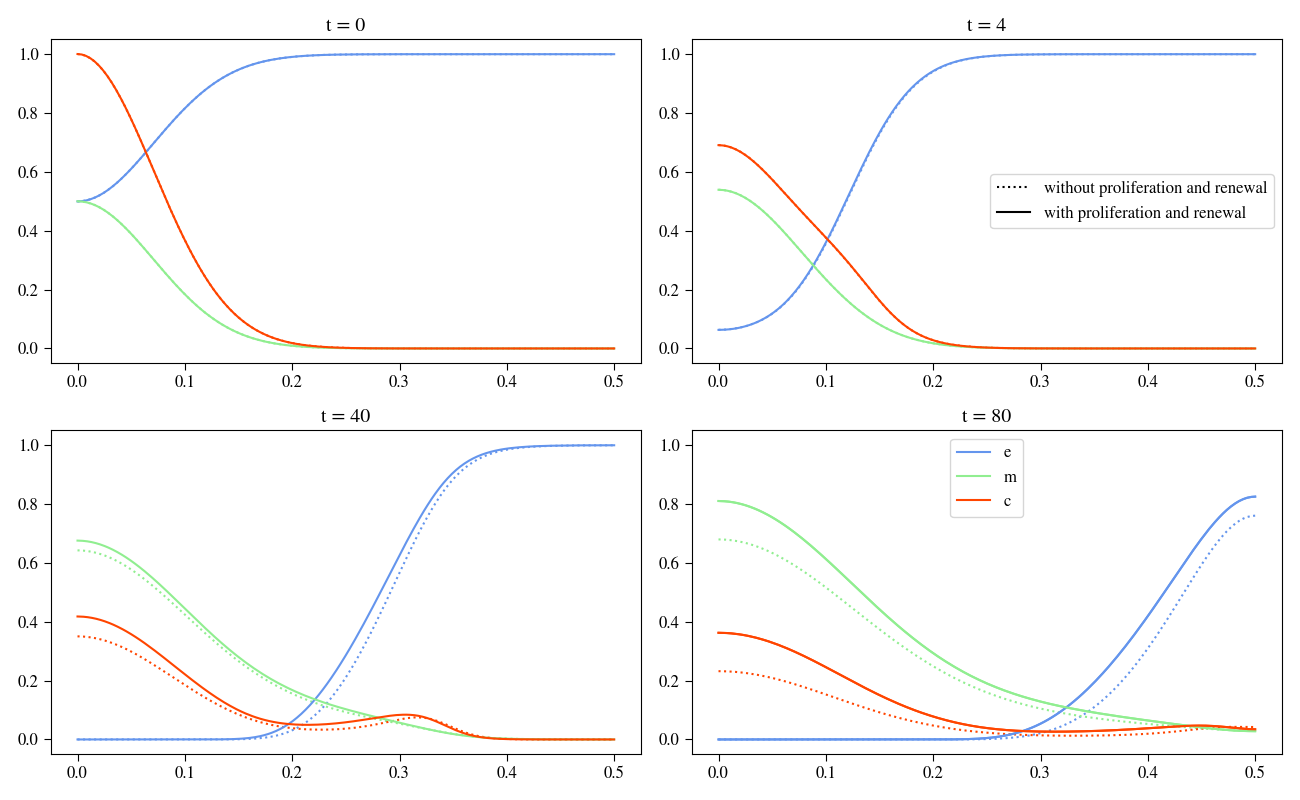
\includegraphics[width=\textwidth]{resources/images/basecase_comparison.png}
    \caption{Describing the updated basecase, in the image above only the updated basecase is plotted, below it is compared to the initial basecase.}
    \label{fig:2D_basecase_comparison}
\end{figure}

Establishing a basecase to compare the following parameter analysis results against it makes sense. In figure~\ref{fig:2D_basecase_comparison}, you can see how introducing tumor cell proliferation and extracellular matrix renewal changes the simulation outcome. For this, we used the values $\mu_1= 0.1$ and $\mu_2=0.5$ according to the only experiment found for this system of equations in the paper of Kolev et al. \cite{Kolev2010}.

Comparing this new basecase to our initial model's basecase, we can see the influences of both $\mu_1$ and $\mu_2$, as the tumor cell density curve is visibly higher than without proliferation, causing a higher production of matrix-degrading enzymes, which would lead to faster ECM degradation. However, this is countered by the renewal factor $\mu_2$ causing the ECM concentration to be higher at the end, at $t=8$, than in the initial basecase experiment.





\subsubsection{Parameter Analysis}

For the Parameter Analysis of the model with proliferation and renewal, we are focusing on comparing the updated model's results with those produced by the model without proliferation and renewal. This will point out again the influence of $\mu_1$ and $\mu_2$ on the system.

\subsubsection*{$d_c$ Variation}
\begin{figure}[h]
    \centering
    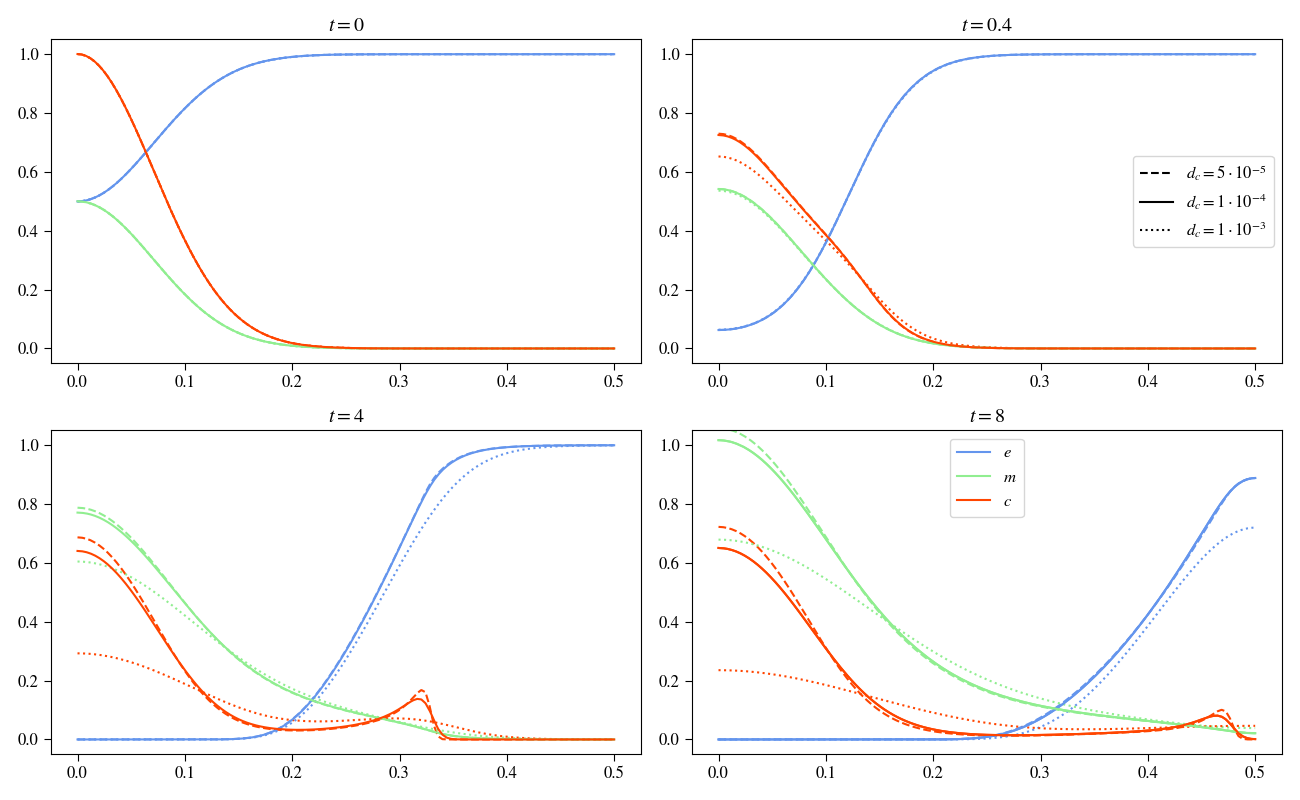
\includegraphics[width=\textwidth]{resources/images/prolif_dc_variation.png}
    \caption{Plots show results for varying $d_c$ whilst keeping the other parameters constant}
    \label{fig:prolif_dc_comparison}
\end{figure}

Varying $d_c$ with proliferation terms, we see the same effects as without proliferation. Higher values for $d_c$ cause a more substantial influence of diffusion and a weaker one for the haptotaxis. This leads to a curve with less or no secondary lump of tumor cells invading the space separately but to a faster distribution process of tumor cells throughout space. The MDE concentration follows this behavior, depending on its production of the tumor cell density distribution in space. The ECM decays faster and the faster the tissue is invaded, the higher the diffusion factor is. Comparing them, we see little differences; only tumor cell density and ECM are raised a little in each plot due to the renewal and proliferation factors, which also causes a higher MDE concentration due to higher tumor cell densities.


\subsubsection*{$\gamma$ Variation}

\begin{figure}[h]
    \centering
    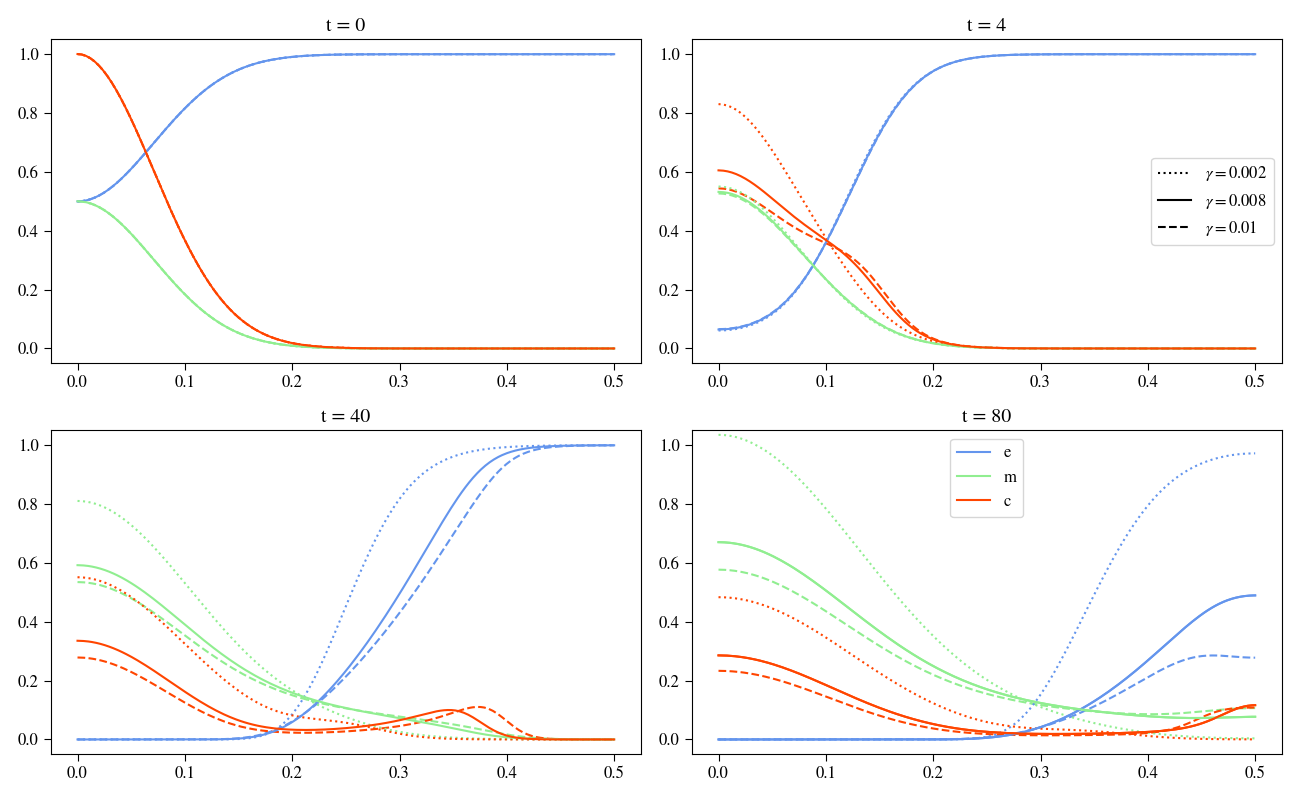
\includegraphics[width=\textwidth]{resources/images/prolif_gamma_variation.png}
    \caption{Plots show results for varying $\gamma$ whilst keeping the other parameters constant.}
    \label{fig:prolif_gamma_variation}
\end{figure}

When we look at $\gamma$, we also can see the same effects as the model without proliferation shows, with the adjustments varying $d_c$, with raised curves for all variables. Increasing $\gamma$ means increasing haptotaxis effects, pulling the tumor cells stronger towards the extracellular matrix molecules. This causes a faster invasion pace and a higher density of tumor cells invading the tissue, but a lower staying at the center at $x=0$. This also means that the ECM degrading process happens faster and the MDEs are more evenly distributed through space the higher $\gamma$ is. As mentioned above, the same effects come in this experiment, introducing proliferation and renewal, with higher values for tumor cell density, MDE and ECM concentration, especially at the later points in time, clearly depictable. Interestingly, by introducing a renewal factor for the extracellular matrix, the proliferation of the tumor cells causes a faster production of matrix-degrading enzymes, which makes the system produce nearly the same results without proliferation and renewal concerning the ECM concentration. Still, introducing the renewal of the ECM results in slightly higher concentrations overall.

\subsubsection*{$\mu_1$ Variation}
The parameter $\mu_1$ describes the proliferation of the tumor cells, using Kolev et al.'s estimate in \cite{Kolev2010} we assume an even distribution with $\mu_1 \sim U[0.1, 1.0]$. Introducing this factor, we can expect a faster production of the matrix-degrading enzymes and a faster degradation of the ECM with an increase in the total amount of tumor cells. Though the effect of the faster ECM degradation might be damped by also introducing a renewal term, we can, especially for higher $\mu_1$ values, expect to dominate the simulations and accelerate ECM degradation.

Since the basecase, using Kolve et al.'s values, sets the proliferation rate of the tumor cells to $\mu_1=0.1$; we consider in the dotted experiment the effects of only introducing the renewal of the ECM.

\begin{figure}[h]
 \centering
 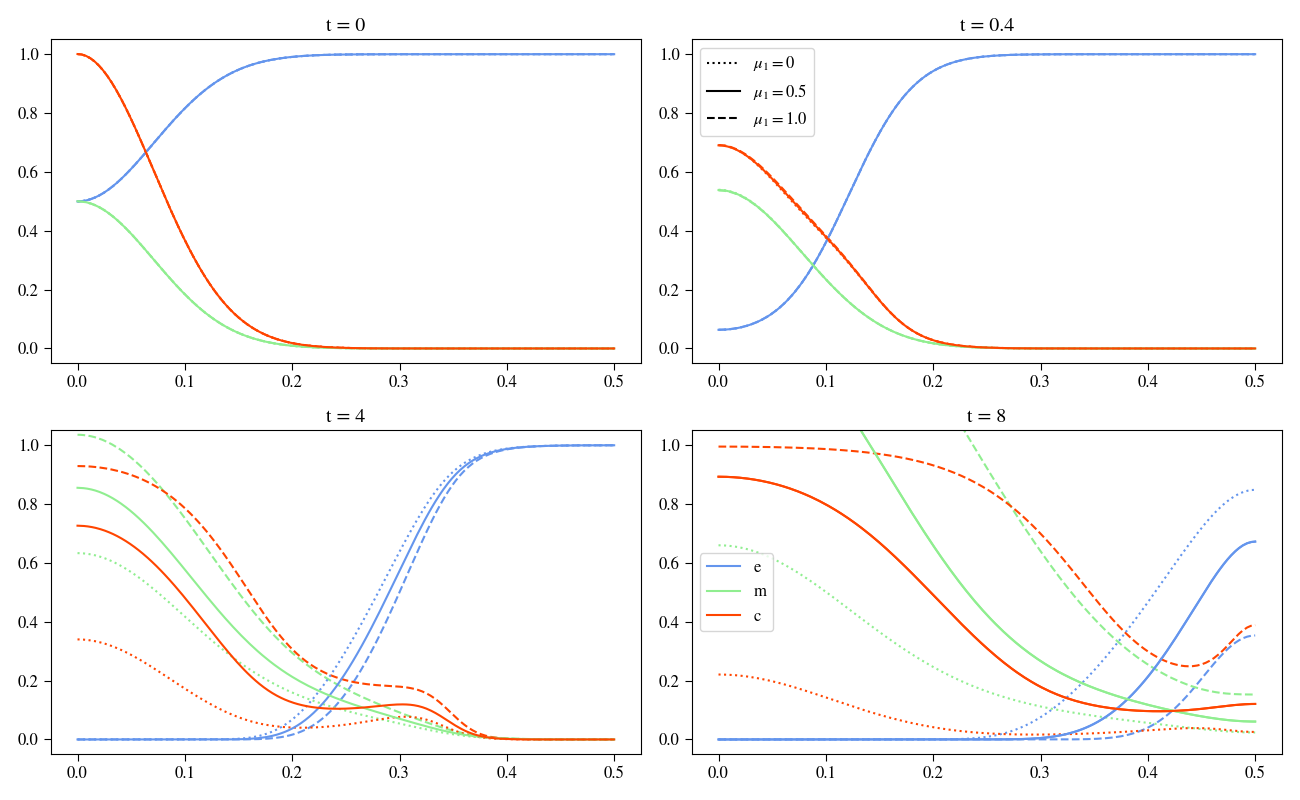
\includegraphics[width=\textwidth]{resources/images/prolif_mu_1_variation.png}
 \caption{Plots show results for varying $\mu_1$ whilst keeping the other parameters constant.}
 \label{fig:prolif_mu_1_variation}
\end{figure}
The effects of $\mu_1$ take some time to act, as we can see no deviations for all the experiments in figure~\ref{fig:prolif_mu_1_variation} at $t=0.4$.

At the next point at $t=4$, the differences are striking concerning all variables. With a higher proliferation factor of the tumor cells, the MDE concentration also rises clearly and the ECM degradation is accelerated. However, at this point, the deviations regarding the curve for the ECM concentration are still subtle.

It looks different at the last point in time, at $t=8$. As mentioned above, an increase in total tumor cells drastically increases the MDE concentration and accelerates the ECM degradation.

Introducing $\mu_1$ means introducing one of the hallmarks of cancer, sustaining proliferative signaling, which makes the tumor cells themselves responsible for producing them instead of requiring other hormones or enzymes to trigger growth signaling. Setting $\mu_1=0$ could result from a drug working, hindering growth signaling.

\subsubsection*{$\eta$ Variation}
\begin{figure}[h]
    \centering
    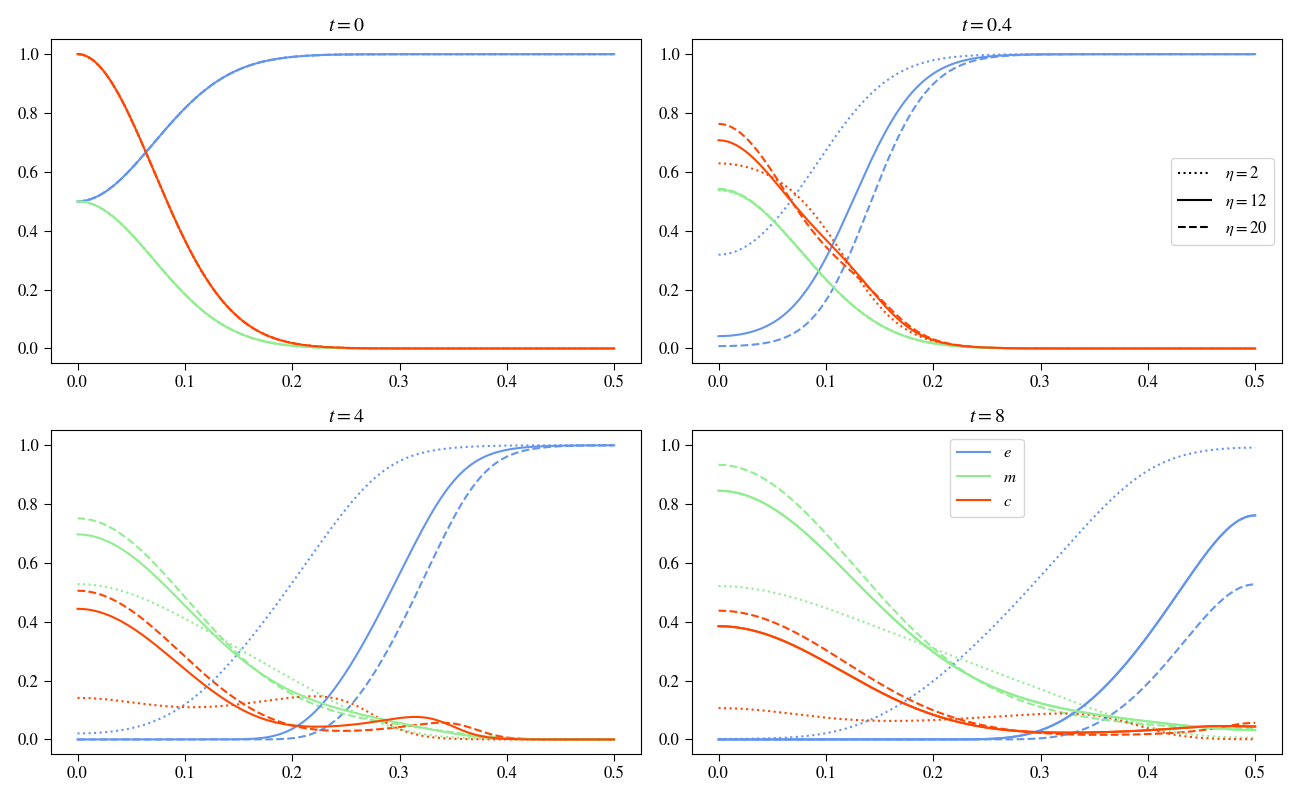
\includegraphics[width=\textwidth]{resources/images/prolif_eta_variation.png}
    \caption{Plots show results for varying $\eta$ whilst keeping the other parameters constant.}
    \label{fig:prolif_eta_variation}
\end{figure}

We see mostly the same effects as we compare the $\eta$ variation between with and without proliferation and renewal models. We see little for the solid and dashed curves, though the new model's curves are all slightly raised. Looking at $\eta=0$, we see some interesting deviations. At the time point $t=0.4$, the plots still look somewhat similar, but looking at $t=4$, we see that the curve of the tumor cells has a more even distribution along the x-axis and also its maximum is visibly lower with the value of about $0.2$ at $x=1.4$ instead of $0.25$ at $x=1.3$. This behavior is due to the renewal of the ECM, where without proliferation, this curve stayed constant throughout the experiment. Here, it can increase, which it does, altering the slope of the curve and, therefore, influencing the haptotatic pull for the tumor cells.
Additionally, the other two experiments showed a visible increase in the tumor cell density and the matrix-degrading enzyme concentration. However, there is only a slight increase in the ECM concentration; here, we can see no increase in area for the tumor cell density. The renewal of the ECM counters the proliferation of the tumor cells and the slowed ECM degrading process. The ECM has visibly increased at the last two points, with both curves of ECM and tumor cells almost mirroring each other. Summing up the areas of both variables, they occupy the space wholly needed for the logistical growth terms. This means that proliferation and renewal will play no more critical role in continuing this experiment as they have reached an equilibrium state and cancel each other out. 


\subsubsection*{$\mu_2$ Variation}
The parameter $\mu_2$ describes the renewal processes of the extracellular matrix molecules. Also, using Kolev et al.'s estimate in \cite{Kolev2010}, we can assume an even distribution with $\mu_2 \sim U[0.1, 1.0]$. In natural processes, the renewal of the extracellular matrix is essential to regulate cell differentiation and wound repair, for example~\cite{Lu2011-yt}.
\begin{figure}[h]
 \centering
 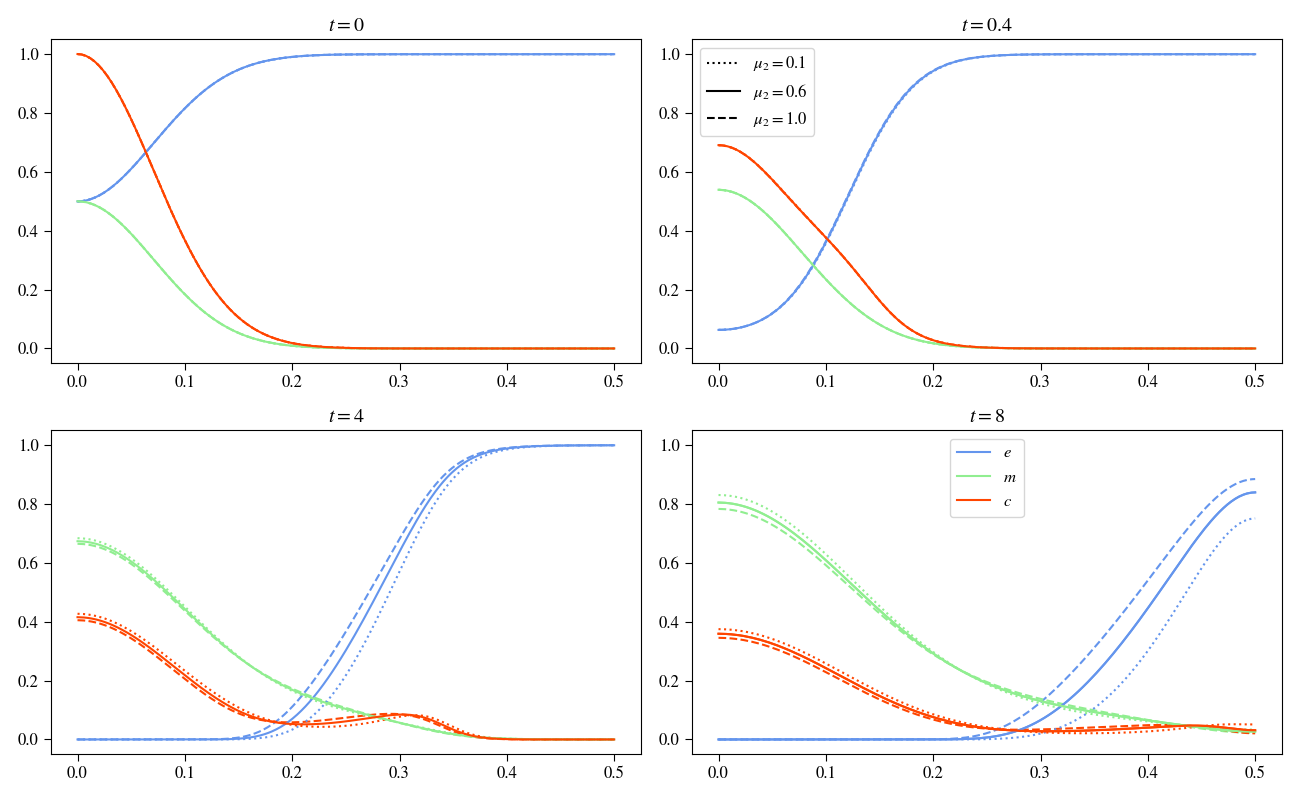
\includegraphics[width=\textwidth]{resources/images/prolif_mu_2_variation.png}
 \caption{Plots show results for varying $\mu_2$ whilst keeping the other parameters constant.}
 \label{fig:prolif_mu_2_variation}
\end{figure}
As we see in figure~\ref{fig:prolif_mu_2_variation}, this renewal process takes some time to show effects. There are no deviations for the experiments after $t=0.4$.

The differences are still subtle when looking at the results later at $t=4$. Increasing $\mu_2$ slows down the extracellular matrix degradation process and affects the motility of the tumor cells, pulling less of them outwards into the surrounding tissue. The MDE concentration nearly overlays completely, with a minimal higher concentration for the lowest $\mu_2$ experiment at the origin due to the slightly higher tumor cell density in this area.

The differences at the last point in time at $t=8$ are still minor compared to varying the other parameters. As mentioned before, the slowed ECM degradation diminishes haptotatic effects, which leads to slightly less matrix-degrading enzyme concentration at the origin.

Varying the ECM renewal rate at this magnitude shows little influence on the resulting simulations.
 
At this point, it is important to say that the renewal rates for tissue in the human body strongly vary. Comparing, for example, bone tissue with connective tissue, we see these processes at highly different time scales. Because we did not have experimental data for this parameter, we only investigated Kolev et al.'s estimates, but considering realistic cases, it is important to have better measures for this parameter.

\subsubsection*{$d_m$ Variation}
\begin{figure}[h!]
    \centering
    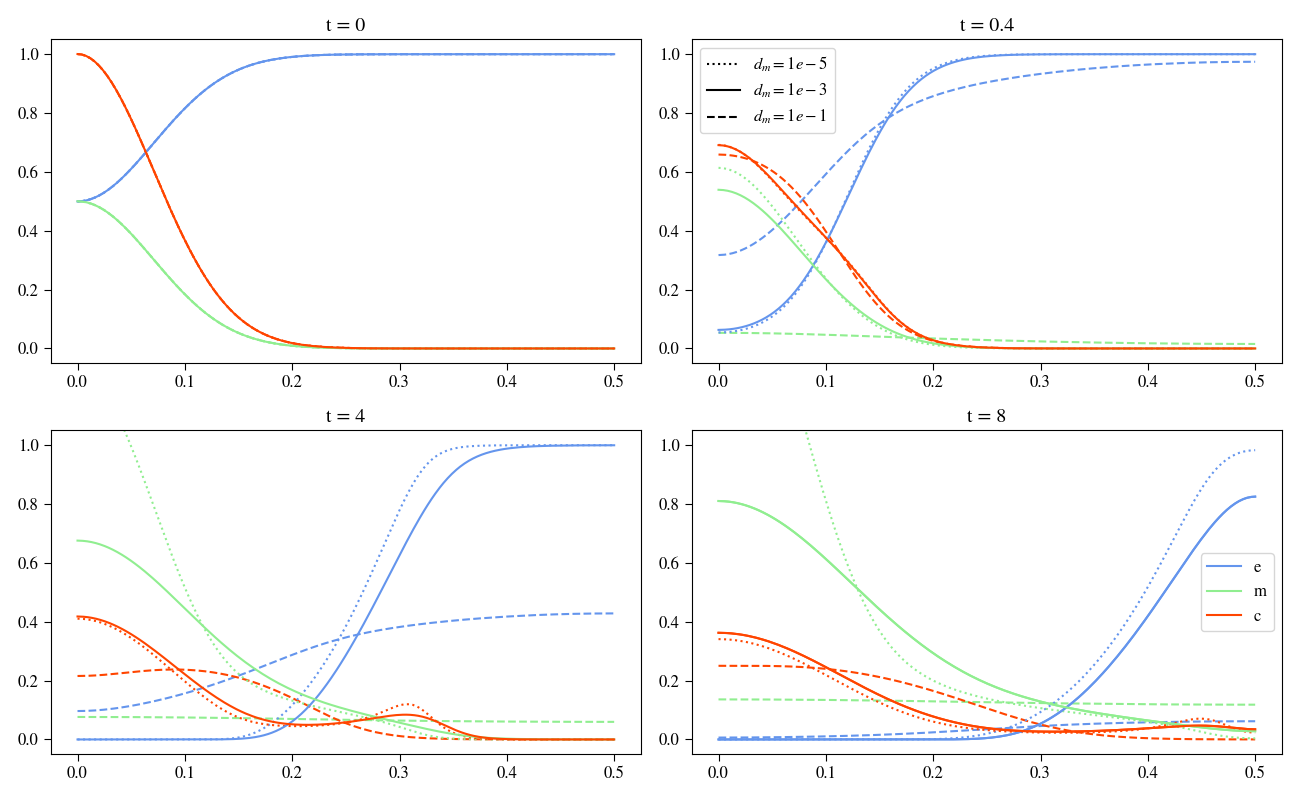
\includegraphics[width=\textwidth]{resources/images/prolif_dm_variation.png}
    \caption{Plots show results for varying $d_m$ whilst keeping the other parameters constant.}
    \label{fig:prolif_dm_variation}
\end{figure}

Comparing the results varying the diffusion factor of the matrix-degrading enzymes does, as before, yield only minor differences between the initial and updated model. As observed before, the tumor cell density curve and the MDE concentration curves are slightly raised due to the proliferation of the tumor cells. However, the ECM curves for the two lower values of varying $d_m$ seem to be subject only to minimal change. We can see that it is raised only for very high values of $d_m$ compared to the model without renewal. The other two curves take off at the same point along the x-axis and finish at the same values for their ECM concentration. Looking at the tumor cell density curves for those $d_m$ values, we see that towards $x=0.5$, they do not describe an as steep bump as the initial model. This also causes a little less MDE concentration, which is responsible for the seemingly unchanged behavior of the extracellular matrix concentration.

\subsubsection*{$\alpha$ Variation}
\begin{figure}[h!]
    \centering
    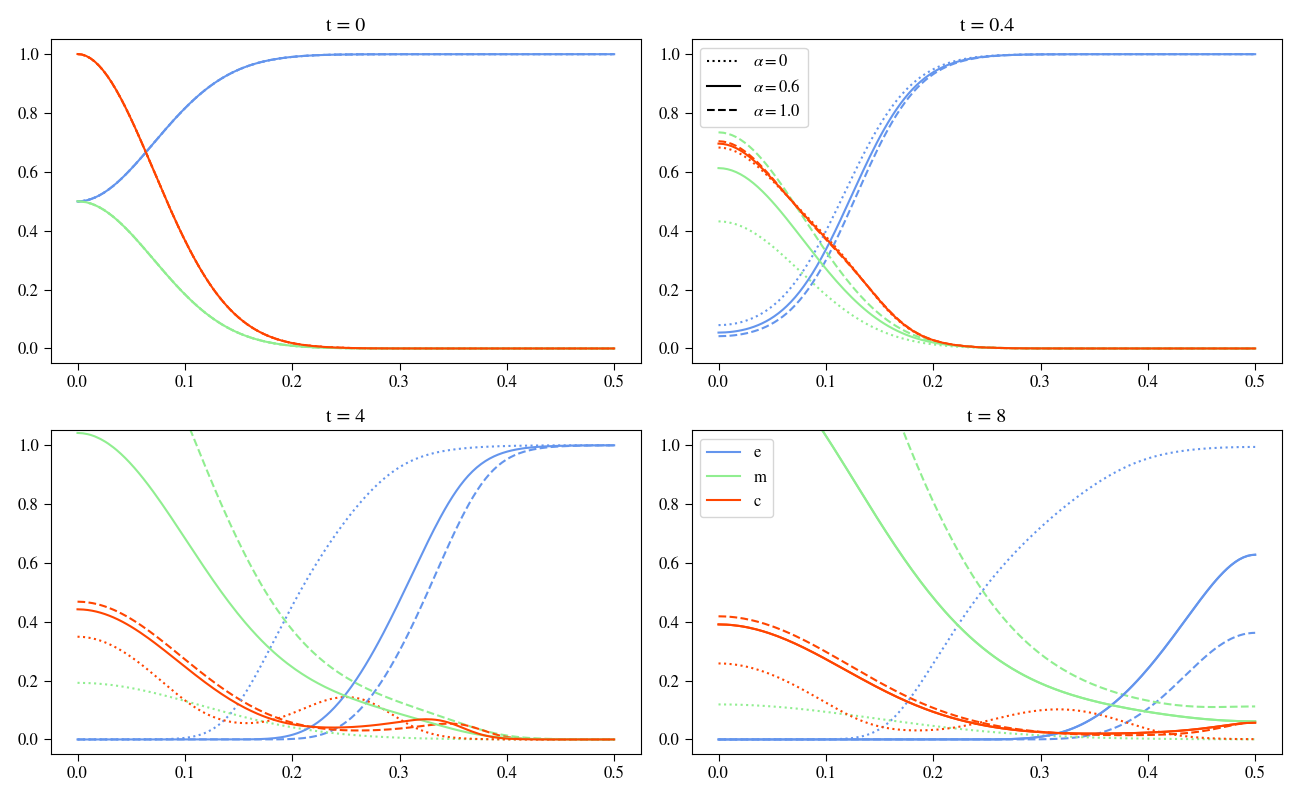
\includegraphics[width=\textwidth]{resources/images/prolif_alpha_variation.png}
    \caption{Plots show results for varying $\alpha$ whilst keeping the other parameters constant.}
    \label{fig:prolif_alpha_variation}
\end{figure}

Taking a look at comparing the $\alpha$-variation yields more exciting results since $\mu_1$ acts as a secondary MDE production effect by producing tumor cells, which in turn produce the matrix-degrading enzymes. Though the overall shape and effects to be observed are the same, after $t=4$, the model with proliferation exceeds one at the origin for the MDE concentration for the two higher $\alpha$ experiments; in contrast, for the model without proliferation, only the one with the highest $\alpha$ value did so. The tumor cell density curve is slightly raised, which allows the MDE concentration. However, the higher values for the MDEs leave the ECM degrading process untouched, with no visible difference between the initial model and the updated one.

\subsubsection*{$\beta$ Variation}
\begin{figure}[h!]
    \centering
    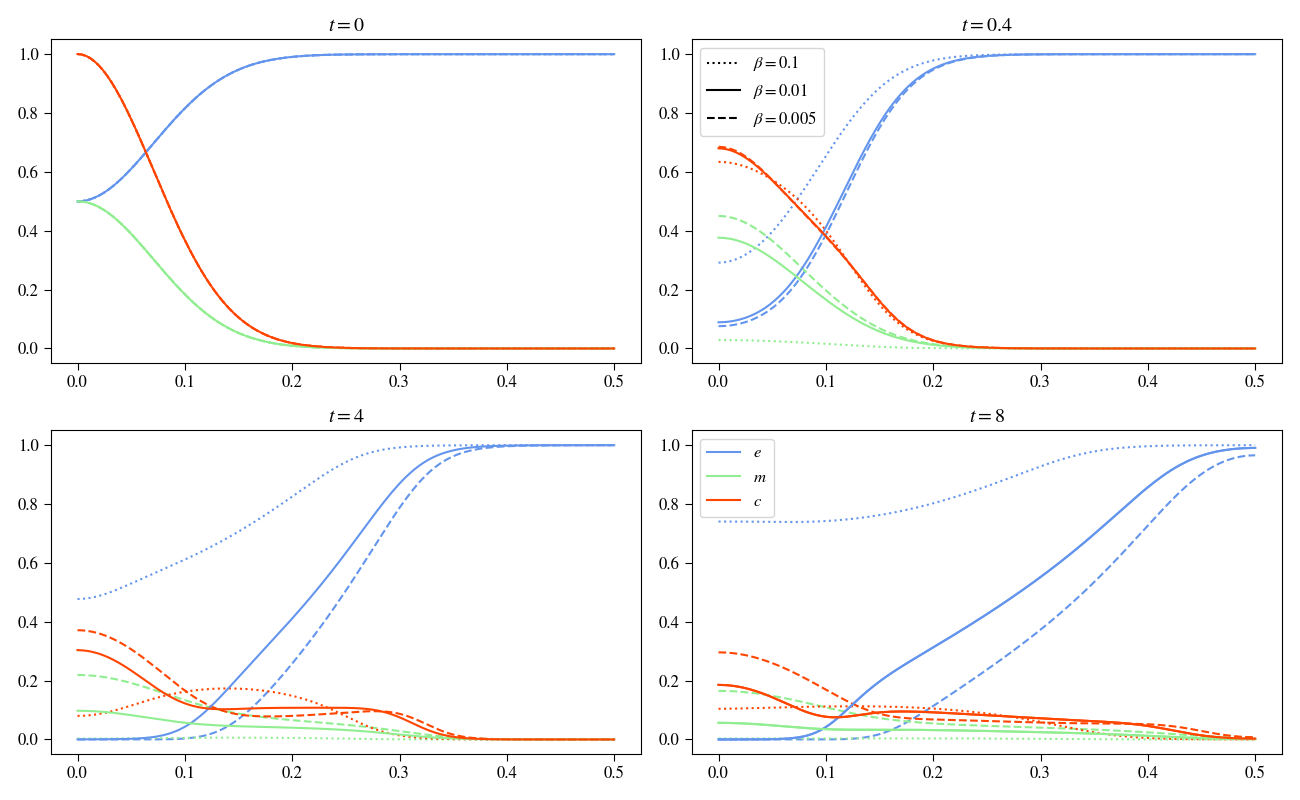
\includegraphics[width=\textwidth]{resources/images/prolif_beta_variation.png}
    \caption{Plots show results for varying $\beta$ whilst keeping the other parameters constant.}
    \label{fig:prolif_beta_variation}
\end{figure}

Considering $\beta$, we can expect that with the introduction of $\mu_2$, the ECM degradation will be slowed considerably with rising $\beta$ since this reduces the MDE concentration and renews the ECM. Looking at the plots, we can see this behavior in the dotted line, which shows the experiment results for the highest $\beta$ value of $0.1$. Though even at the end, it has an overall area that is slightly less than the initial condition, we can see going from timestep $t=0.4$ to $t=4$ that MDE decay and ECM renewal were sufficiently strong to restore the ECM and going from $t=4$ to $t=8$ we see this behavior again, renewing the ECM. The other two experiments for $\beta$ showed no effects as strong as with $\beta=0.1$. However, we can still see the effects of proliferation and renewal especially clear in the solid line, $\beta=0.01$, at the last point in time, where we can observe a visible increase of both ECM and tumor cell density. In this experiment, we see that $\beta$ is a little too low to counter the effects of ECM degradation; going from $t=4$ to $t=8$, we see an apparent decline of ECM concentration, though it is not as striking as for $\beta=0.005$. 

\subsubsection*{Cross-Variation}

\subsubsection*{$\mu_1 - \mu_2$ Variation}
\begin{figure}[h!]
    \centering
    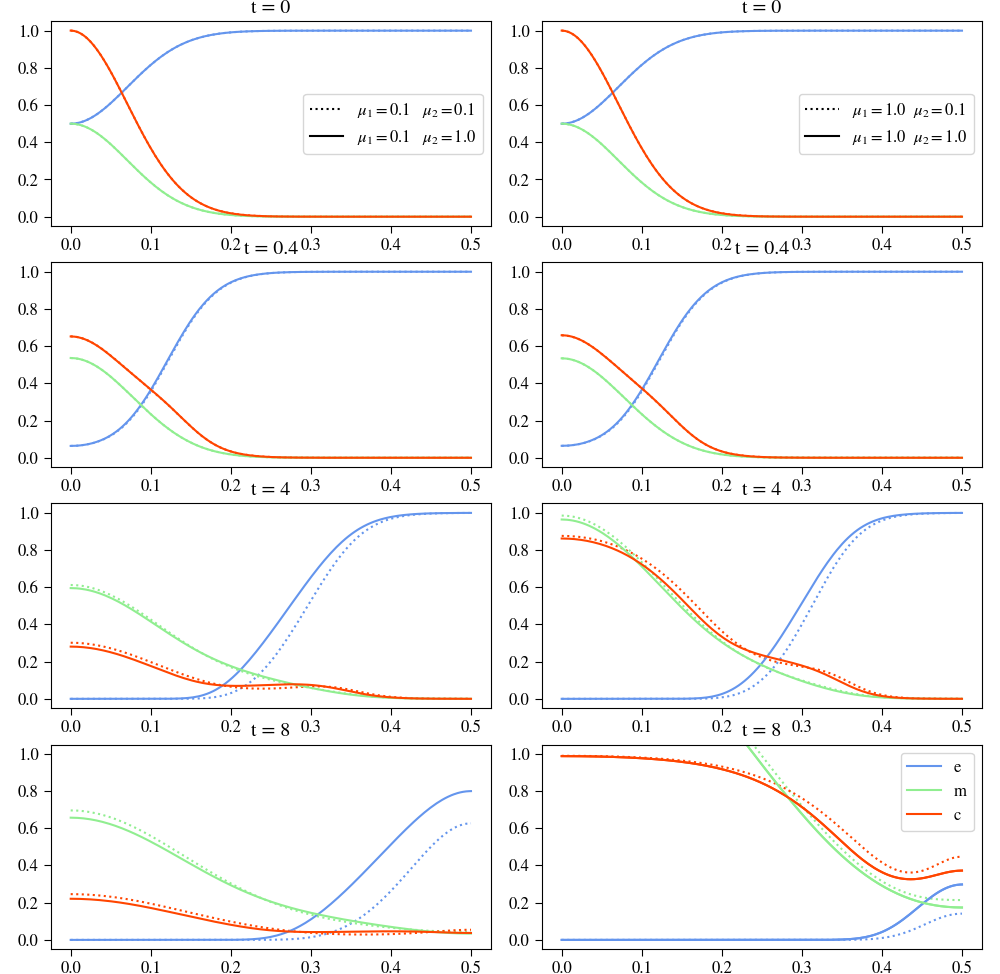
\includegraphics[width=\textwidth]{resources/images/prolif_mu_1_mu_2_variation.png}
    \caption{Plots show results for varying both $\mu_1$ and $\mu_2$ whilst keeping the other parameters constant.}
    \label{fig:prolif_mu_1_mu_2_variation}
\end{figure}
The effects of observing this cross variation take some time, as did the separate variations of both $\mu_1$ and $\mu_2$. For both $\mu_1=\mu_2=0.1$, we see that slower ECM renewal and slower tumor cell proliferation increase the degrading process of the extracellular matrix and, with this, affect the haptotaxis effect to increase slightly. At the center, a lump remains that has a maximum higher than for the experiment with $\mu_2=1.0$ and the invasion of the tissue has proceeded faster. Increasing $\mu_2$, as previously mentioned, results in slower ECM degradation due to the increased renewal term and therefore, the tumor cells are stretched out more evenly along the x-axis. Looking at the results when increasing $\mu_1$, we also see the effects only after $t=4$. For $\mu_2=0.1$, we see that the tumor cell density at $x=0$ is slightly more significant and at $x\approx 2.9$, the curve for $\mu_2=0.1$ is also slightly larger, being a little below $\mu_2=1.0$ in between $x\approx 0.2$ and $x\approx 0.29$. The curve for the MDEs looks very similar in both cases for $\mu_2$ due to the very similar tumor cell density curve, c, though the eECM has visibly faster degraded for $\mu_2=0.1$ due to the slower renewal.

\subsubsection*{$d_c - \gamma - \mu_1$ Variation}
\begin{figure}[h!]
    \centering
    \adjustbox{width=\textwidth}{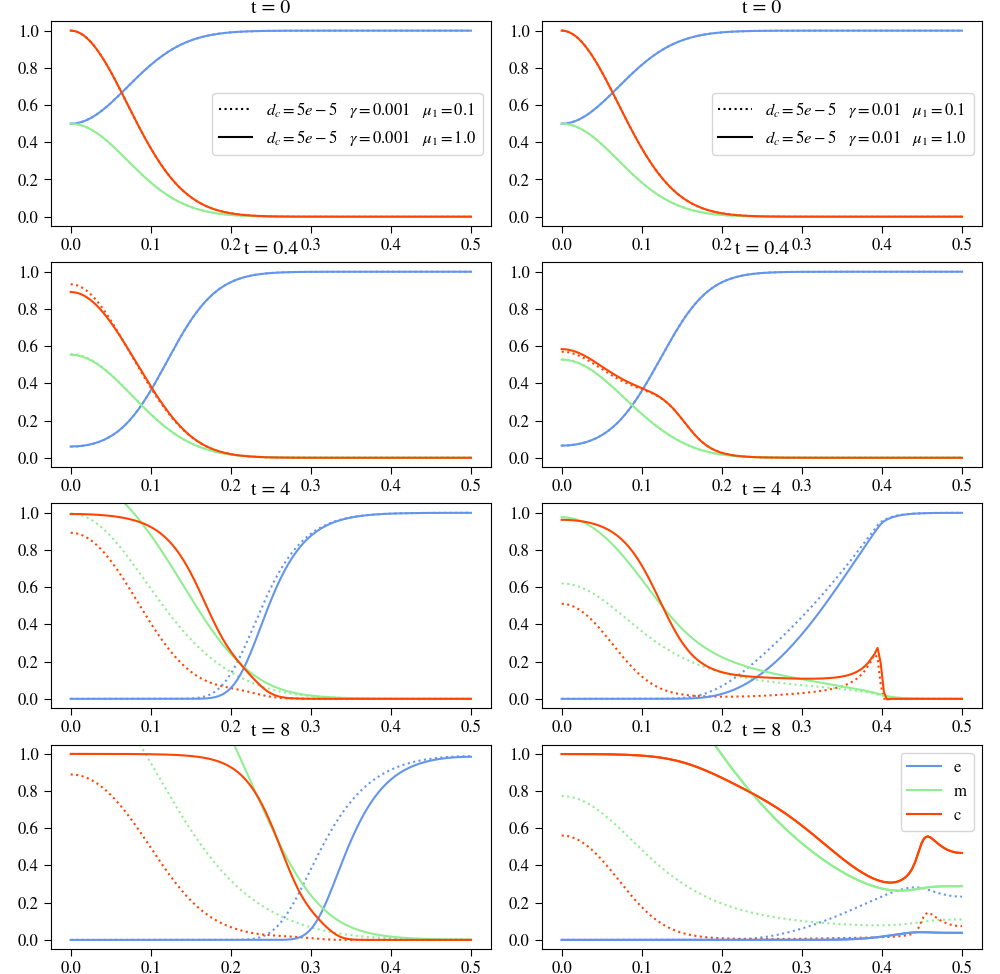
\includegraphics{resources/images/prolif_dc_gamma_mu1_1.png}}
    \caption{Plots show results for varying both $d_c$, $\gamma$ and $\mu_1$ whilst keeping the other parameters constant. This plot is the first of two, with the same $d_c$ value for every plot in this figure.}
    \label{fig:prolif_dc_gamma_mu_1_variation_1}
\end{figure}

\begin{figure}[h!]
    \centering
    \adjustbox{width=\textwidth}{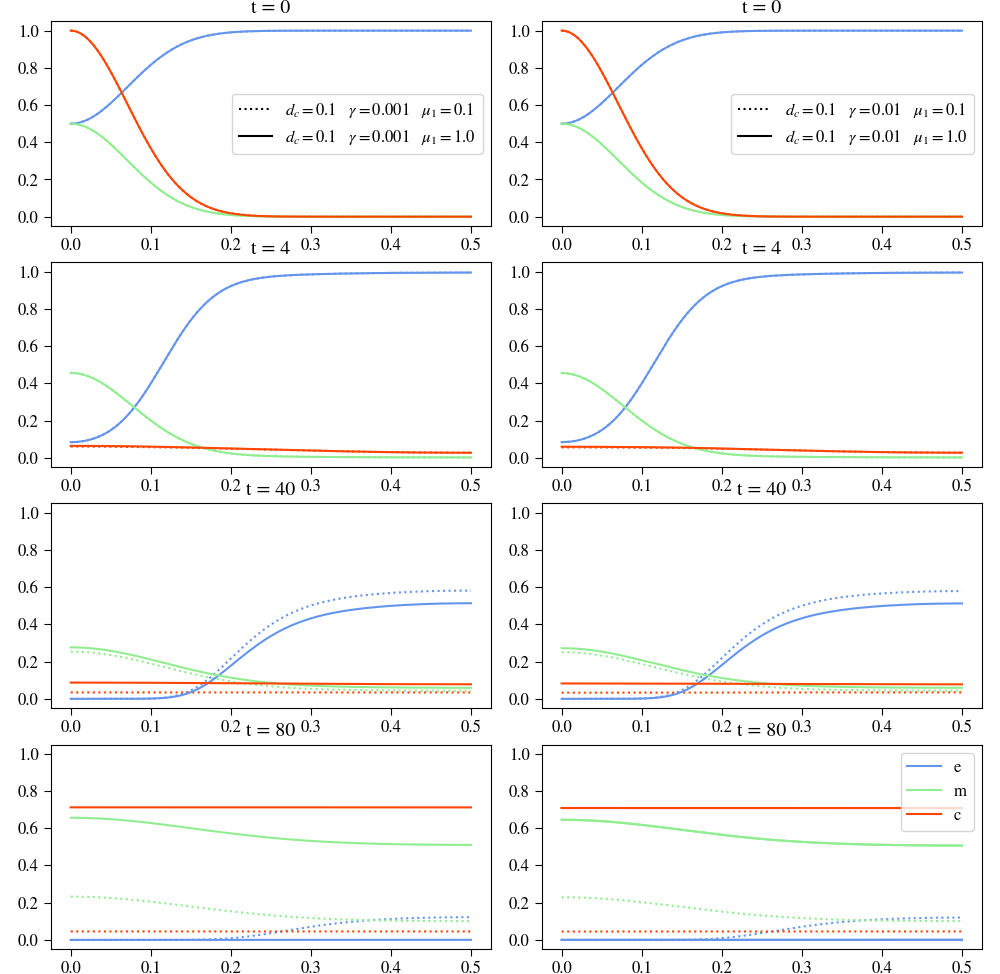
\includegraphics{resources/images/prolif_dc_gamma_mu1_2.png}}
    \caption{Plots show results for varying both $d_c$, $\gamma$ and $\mu_1$ whilst keeping the other parameters constant. This plot is the second of two, with the same $d_c$ value for every plot in this figure.}
    \label{fig:prolif_dc_gamma_mu_1_variation_2}
\end{figure}

First we are going to take a look at how chaning $\gamma$ and $\mu_1$ affects the system whils having lower diffusion values for the tumor cells as the basecase value with $d_c=5\cdot 10{-5}$. Figure~\ref{fig:prolif_dc_gamma_mu_1_variation_1} shows the results of these experiments. Inspecting the dotted curve on the left side column, shows the results for all parameters set to low, we see that diffusion is tha mian factor for the movement of the tumor cells, with only little influence of haptotaxis, the tumor cells staying with their maximum at the center. Becasue fo this we also get a high MDE concentration there, but very little excedding the region past $x=0.3$. Due to the MDE also staying centered around thr origin the ECM there is completely degraded, though at $x=0.4$ and further still completely there. Increasing the proliferation factor to $\mu_1=1.0$ shifts the tumor cell density rightwards, making proliferation also a factor for the cell density movement, though keeping the same shape as the low proliferation factor experiment. This right shift causes the MDE concentration to also shift to the right, leading to a faster ECM degradation. Comparing these two experiments already shows the influence of proliferation.

Taking now a look at the right column in figure ~\ref{fig:prolif_dc_gamma_mu_1_variation_1} we see the effects of increased $\gamma$ to $\gamma=1.0$. Foremost we see for the tumor cell density a leading edge developing, seperating it into two lumps, with one staying at the center the other invading the tissue and staying where $\nabla (c \nabla e)$ is highest. With increased $\mu_1$ this division moving into the tissue is getting more pointy, defying differentiability. After $t=4$ we can observe clear differences regarding ECM and MDE concentration. We see that for higher $\mu_1$ we also get a higher MDE concentration which degrades the ECM visibly faster at the end of the experiments at $t=8$. Though interestingly at $t=4$ the ECM degradataion difference is only minor, at the last point in time the accellerated tumor cell proliferation shows its effet with producignmore MDEs and degrading the ECM considerably faster. What is also interesting to note is that increasing $\gamma$ and keeping $\mu_1$ low the total area of the MDE concentration is lowered also.
Increasing now $d_c$ to $0.1$ we see for all experiments in figure~\ref{fig:prolif_dc_gamma_mu_1_variation_2} that the diffusion of the tumor cells was sufficiently high to evenly distribute the tumor cells constatnly in the space. This constant distribution allows to get an even better look at how $\mu_1$ affects the results, by seeing the lines, describing the tumor cells, rise through time. Looking at the tumor cells over time we can see no observable difference for varying $\gamma$. Haptotaxis effects are completely overlaid by diffusion. We see in the left column that if keeping dc high and $\gamma$ low, but increasing $\mu_1$ leads to higher MDE production rates and also faster ECM degradation. The same behaviour is observable in the right column showing the results for high $\gamma$. That we see no difference is clear, since the tumor cell density development is identical over time as mentioned above. 



\subsubsection*{$\eta -\mu_2$ Variation}
\begin{figure}[h!]
    \centering
    \adjustbox{width=\textwidth}{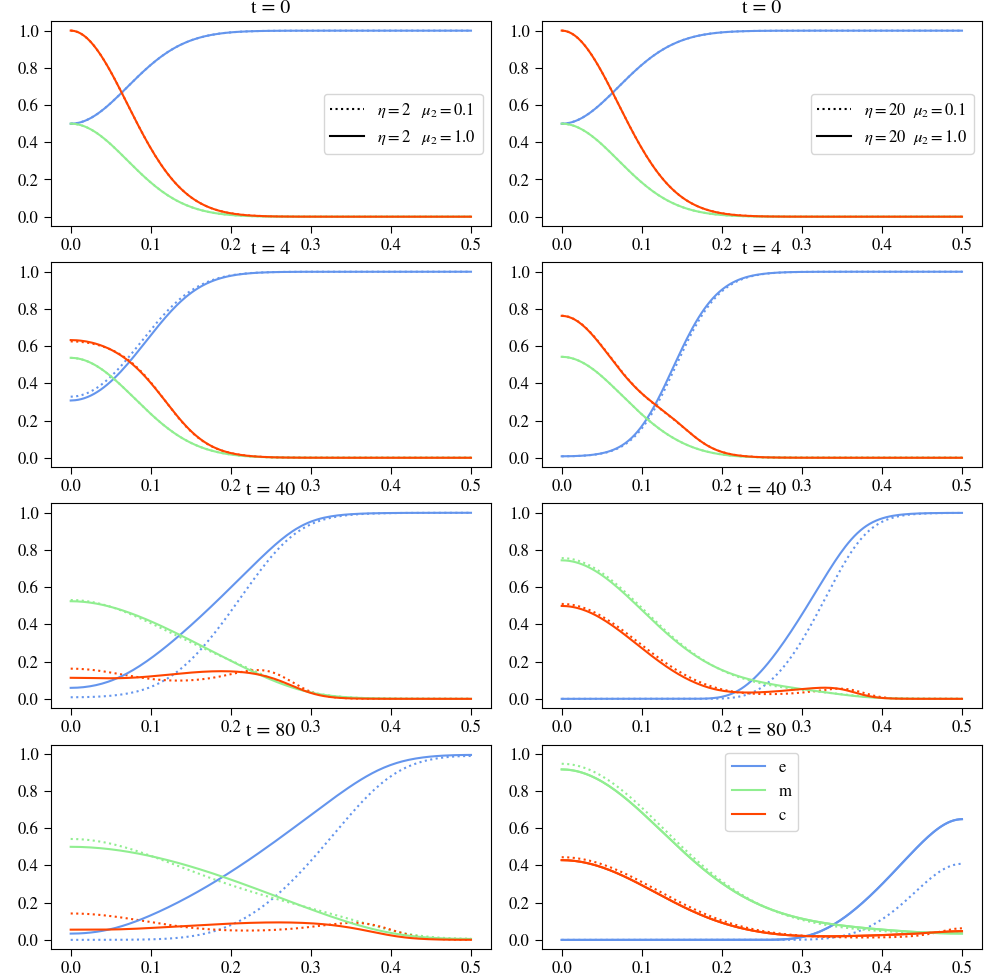
\includegraphics{resources/images/prolif_eta_mu2_variation.png}}
    \caption{Plots show results for varying both $\eta$ and $\mu_2$ whilst keeping the other parameters constant.}
    \label{fig:prolif_eta_mu_2_variation}
\end{figure}

Varying both $\eta$ and $\mu_2$, we can expect apparent changes in the curve describing the ECM concentration. On the left side of figuer~\ref{fig:prolif_eta_mu_2_variation}, we see the two experiments for low $\eta$ values and that increasing $\mu_1$ has only a little effect. Where we could have expected to see an increase of the ECM, maybe even, we see that the ECM curves for both experiments verify that the renewal factor $\mu_2$ was too low to counter the ECM degradation, even with a low degradation factor. Still, between $\mu_2=0.1$ and $\mu_2=1.0$, there are visible differences in the degrading speed of the ECM. We can also observe that with the higher renewal term, the tumor cell density curve receives more of an effect of haptotaxis, resulting in a more stretched curve with only one long lump of tumor cells, whereas, for the lower renewal factor, we can still clearly see that there is a division that invades the tissue and one that stays at the origin. Concerning the MDE curves, we see little difference for higher $\mu_2$, which means more stretched tumor cell density. We can also observe a more stretched MDE curve with a lower maximum at the origin. 

Looking at the experiments with raised $\eta$ to accelerate the ECM degrading process, we can only see pregnant differences in the curve describing the ECM concentration; the other two look across the steps in time to be widely similar. For the ECM curve, we see that the experiment with the lower $\mu_2$ value results in a faster degradation process.






\subsection{2D Results with Proliferation and Renewal - Heterogenous ECM}
\label{sec:2D_heterogenous_ECM}
\begin{figure}[h!]
 \centering
 \adjustbox{width=0.95\textwidth}{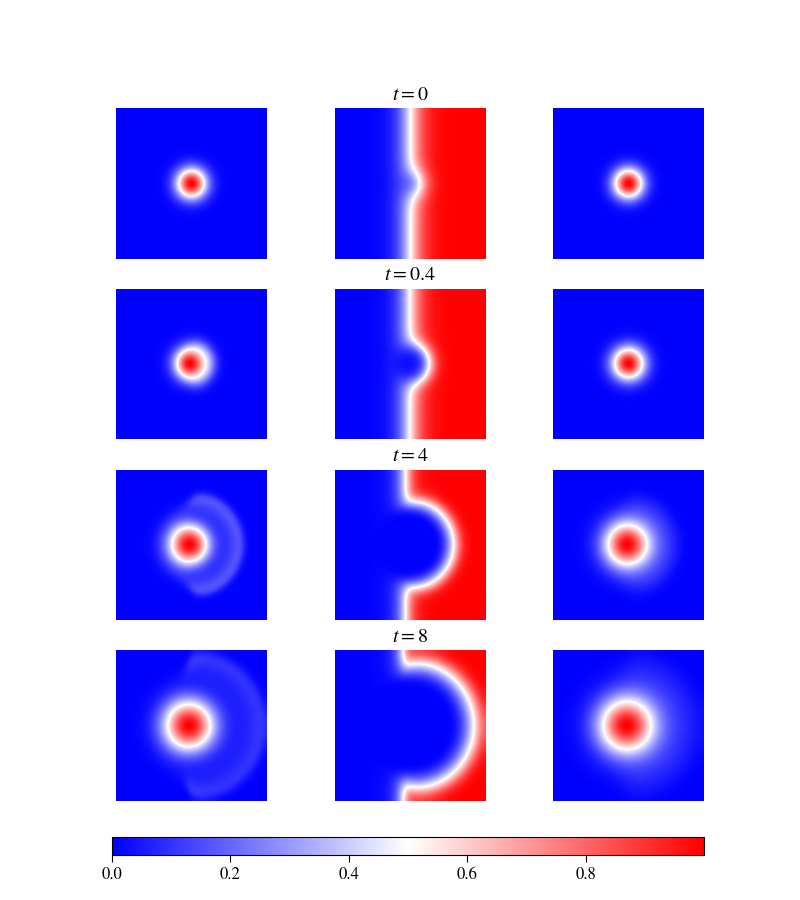
\includegraphics{resources/images/2D_heterogenous_ECM.png}} 
 \caption{2D Results using a heterogenous ECM with the parameter values: $d_c=5\cdot 10^{-4}$, $\gamma=0.0055$, $\mu_1 = 0.1$, $\eta=10$, $\mu_2=0.5$, $d_m = 1\cdot 10^{-3}$, $\alpha = 0.3564$, $\beta = 0$; left: tumor cell density, middle: ECM concentration, right: MDE concentration.}
 \label{fig:2D_heterogenous_ECM}
\end{figure}
Figure~\ref{fig:2D_heterogenous_ECM} you can see the effects using a heterogenous extracellular matrix structure. The plots show the tumor cell density in the left column, the extracellular matrix concentration in the middle column and the matrix-degrading enzyme concentration on the right. For the parameters, we assumed the basecase studying the model with proliferation. 

This experiment describes a more realistic biological scenario, as seen in figure~\ref{fig:tumour_invasion_stage}, where the tumor cells are located at the basement membrane of neighboring tissue and have degraded this membrane to invade the surrounding tissue and degrade the extracellular matrix.

The first image in the middle column shows the experiment's initial distribution. The extracellular matrix molecule concentration is only on the right side of the plot, which indicates that neighboring tissue has been invaded. In the center of the same image, there is a hollow spot where the tumor cells of the initial distribution are located. 

After four time steps, the ECM slowly degrades and the tumor cells are pulled further into the neighboring tissue by haptotaxis caused by the ECM structure. The concentration of the matrix-degrading enzymes shows little difference in their behavior compared to the experiments done with a homogenous ECM. They only depend indirectly on the ECM by being produced where the tumor cells are being pulled by the extracellular matrix concentration. 

The next point shows increased ECM degradation, further invading tumor cells into the tissue. The tumor cells behave as a semicircular wave moving into the direction of the ECM; the primary lump remains at the center, with the edge of having containing a smaller amount of cells moving outwards. The image describing the matrix-degrading enzyme concentration still shows only minor effects; looking closely, we can see that from the center moving to the right, there is a slightly higher concentration than in the other direction.

The last row depicts the experiment after $t=8$ timesteps and the above mentioned effects are propagated. The ECM degradation has continued, as has the invasion of the tumor cells. The wave moving in the direction of the remaining extracellular matrix molecules has spread through space, decreasing its strength. The MDEs still show little influence on the heterogeneous ECM structure, with the primary lump staying centered and only making it difficult to recognize more concentration towards the movement of the tumor cells and concentration of the extracellular matrix.
 
Considering different extracellular matrix molecules and structures or physical influences such as heat or radiation, the ECM structure and the system's behavior can be adjusted to simulate better real-life scenarios of cancer invading tissue.
